\def\year{2017}\relax
%File: formatting-instruction.tex
\documentclass[letterpaper]{article}
\usepackage{aaai17}
\usepackage{amsmath}
\usepackage{amsthm}
\usepackage{times}
\usepackage{helvet}
\usepackage{courier}
\usepackage{graphicx}
\usepackage{subfigure}
\usepackage{mdwmath}
\usepackage{mdwtab}
\usepackage{amssymb}
\usepackage{booktabs}
\usepackage{algorithm}
\usepackage{pifont}
\usepackage[noend]{algpseudocode}
\usepackage{balance}
\usepackage{bm}
\usepackage{ulem}
\usepackage{array}
\usepackage{balance}
\usepackage{multirow}
\usepackage{multicol}
\usepackage{threeparttable}
\frenchspacing
\setlength{\pdfpagewidth}{8.5in}
\setlength{\pdfpageheight}{11in}
\usepackage[marginal]{footmisc}

\setcounter{secnumdepth}{0}  
 \begin{document}
% The file aaai.sty is the style file for AAAI Press 
% proceedings, working notes, and technical reports.
%
\title{A General and Fine-grained Analysis of the Variance Reduction Technique in SVRG and a Novel Acceleration Method}
%\author{
%}
\maketitle
\begin{abstract}
Stochastic gradient descent (SGD) with variance reduction  technique such as SVRG is efficient to train parameters of many machine learning algorithms. Although many variants of SVRG have been proposed,  the analysis of variance has not been thoroughly discussed. Besides,  the variants of SVRG have to keep a snapshot of the full gradient in every epoch, which is computationally expensive. In this paper, we propose a general framework EUI  to unify the existing variants of SVRG, and then  provide a general and fine-grained analysis of the variance from a new prospective. Moreover,   a new variant of SGD with the variance reduction technique named \textsc{sampleVR} is proposed. \textsc{sampleVR} replaces the full gradient computation with an estimation, thus decreasing gradient complexity significantly.  Both the theoretical analysis and the empirical studies show that \textsc{sampleVR} makes  training loss converge faster than its counterparts obviously. 
\end{abstract}

\section{Introduction}
\label{sect_introduction}
Many machine learning problems such as classification and regression  can be  presented as the optimisation problem described by Equation \ref{equa_loss_minimization}. $F(\omega)$ denotes the training loss or the loss function which is the sum of the finite functions, i.e. $\nabla f_i(\omega)$ with $i\in\{1,2, ..., n\}$. $\omega$ is the parameter of the machine learning model, and $n$ represents the size of the training data. $R(\omega)$ is the regulariser  which is used to prevent overfitting.    

\begin{equation}
\label{equa_loss_minimization}
\min F(\omega),~~~~~F(\omega)=\frac{1}{n}\sum\limits_{i=1}^n f_i(\omega)+R(\omega)\\
\end{equation}

Gradient descent (GD) is used to train the parameters for such underlying machine learning problems. Since GD computes a full gradient every iteration, it performs a large amount of gradient calculations.  This would affect the performance significantly in the presence of a large amount of training data. The stochastic gradient descent (SGD) overcomes the weakness of GD by using a stochastic gradient instead of the full gradient to train parameter. However, variance caused by the stochastic gradient usually impairs convergence of the training loss. Specifically, when the parameter is close to the optimum, it is increasingly difficult to make a further progress  due to the variance. Conventional studies show that a decaying learning rate can be used to decrease the variance. But the training loss converges slowly when the learning rate is small. 

Recently, Johnson et al. improve SGD with the variance reduction technique named SVRG which uses a constant learning rate to train the parameter \cite{Johnson:9MAvkbgy}.  Based on the variance reduction technique adopted by SVRG, many variants of SVRG such as S2GD \cite{Richtarik:2013te}, mS2GD \cite{Liu:2015bx}, EMGD \cite{Zhang2013Linear}, SVR-GHT \cite{Li:2016vh}, Prox-SVRG \cite{Xiao:2014vw}, SVRG++ \cite{Allen2015Improved}, and Katyusha \cite{Allenzhu2016Katyusha} have been proposed. However, the analysis of the variance, which is essential to understand and exploit the variance reduction technique, lacks enough discussion. Although Zeyuan et al.  present an upper bound of the variance, this  achievement is obtained with many  simplifications \cite{AllenZhu:2016up}. Moreover, those existing algorithms are organised by epochs. One epoch consists of some iterations. SVRG and its variants have to keep a snapshot of the full gradient for every epoch, leading to a large amount of gradient calculations. When the size of the training data is huge, the snapshot of the full gradient is extremely time-consuming.   In short, it is meaningful to give a quantitative analysis  of the variance in general settings so that the potential of the variance reduction technique can be exploited.  Additionally, if the snapshot of the full gradient in an epoch can be avoided, SVRG and its variants will be accelerated a lot, which results in a better performance of the convergence.
 
As an important improvement of SVRG and its variants, we provide a thorough analysis about the variance from a new prospective. To present the analysis, we propose  a general framework named EUI, and then perform the analysis under the framework. The  update rule of the parameter in the variance reduction technique can be divided into three aspects, including the variance source, the variance reducer and the progressive direction. The variance reducer is the real reason to reduce the variance.  More specifically, we provide both lower and upper bounds of the variance, and then analyse improvement of the variance reduction in the existing variants of SVRG.   Moreover, a new variant of SGD with the variance reduction technique denoted by \textsc{sampleVR} is proposed, which replaces the snapshot of the full gradient by using an unbiased estimation, and accelerates the convergence of the training loss.  The contributions of the paper are outlined as follows:
\begin{itemize}
\item A general framework, i.e. EUI is proposed to unify the existing variants of SVRG. 
\item The variance caused by the stochastic gradient is analysed in the underlying framework. Both lower and upper bounds of the variance are presented in general settings.
\item A new variant of SGD with the variance reduction technique, i.e. \textsc{sampleVR} is proposed, which achieves a linear convergence rate with low gradient complexity.
\item Extensive evaluation tests show that \textsc{sampleVR} outperforms  other previous work significantly. 
\end{itemize}

To keep the paper reasonably concise, a list of symbols   used in the paper and the proofs are given in support materials. The paper is organised as follows. Section \ref{sect_related_work} reviews recent related work about SGD with the variance reduction technique. Section \ref{sect_framework}  presents the general framework, i.e. EUI, and then provides the analysis of the variance reduction under the framework. Section \ref{sect_sample_vr} presents a new reduced variance SGD, i.e. \textsc{sampleVR}, and provides the theoretical analysis of both the performance of convergence and the gradient complexity.   Section \ref{sect_performance_evaluation} demonstrates the extensive performance evaluations to verify our theoretical analysis. Section \ref{sect_conclusion} concludes this paper. 


%In order to keep the paper reasonably concise, we present  the meanings of symbols used in the paper and the proofs in support materials. The paper is organised as follows. Section \ref{sect_related_work} reviews recent related work about SGD with the variance reduction technique. Section \ref{sect_framework}  presents the general framework, i.e. EUI which unifies  the existing variants of SVRG, and then provides the analysis of the variance  under the framework. Section \ref{sect_sample_vr} presents a new reduced variance SGD, i.e. \textsc{sampleVR}, and provides the theoretical analysis of both the performance of convergence and the gradient complexity.   Section \ref{sect_performance_evaluation} demonstrates the extensive performance evaluations to verify our theoretical analysis. Section \ref{sect_conclusion} concludes this paper. 
 

\section{Related work}
\label{sect_related_work}
Various variants of  SGD with the variance reduction technique have been proposed, including SAG \cite{Schmidt:2013ui}, SAGA \cite{Defazio:2014vu}, SDCA \cite{ShalevShwartz:2016vy}, and SVRG \cite{Johnson:9MAvkbgy} and its variants and so on. It is noting that SAG, SAGA and SDCA adopt different variance reduction techniques from SVRG and its variants. Although variance reduction techniques used in SAG, SAGA and SDCA are competitive with that of SVRG and its variants,  this paper focuses on the variance reduction technique used in SVRG and its variants. To the best of our knowledge,  the variants of SVRG includes S2GD \cite{Richtarik:2013te}, mS2GD \cite{Liu:2015bx}, EMGD \cite{Zhang2013Linear}, SVR-GHT \cite{Li:2016vh}, Prox-SVRG \cite{Xiao:2014vw}, SVRG++ \cite{Allen2015Improved}, and \textsc{CheapSVRG} \cite{Shah2016Trading}. 

Zeyuan et al. have presented an upper bound of the variance caused by the stochastic gradients when using the variance reduction technique \cite{AllenZhu:2016up}. Such upper bound of the variance is subject to  many simplifications. Our analysis about the variance is a complement to that work, which is obtained in general settings, and does not require the simplifications assumed in that work. Vatsal et al. have proposed \textsc{CheapSVRG} which uses sampled instances to estimate the full gradient \cite{Shah2016Trading}. The number of those sampled instances is a parameter which needs to be identified before running of \textsc{CheapSVRG}. Comparing with \textsc{CheapSVRG}, our proposed algorithm, i.e. \textsc{sampleVR} does not need to tune extra parameters. Additionally, although both \textsc{CheapSVRG} and \textsc{sampleVR} can achieve a linear convergence rate, the analysis of \textsc{CheapSVRG} is obtained with two extra strong assumptions, which are not required in \textsc{sampleVR}. Furthermore, extensive empirical studies show that  \textsc{sampleVR} outperforms \textsc{CheapSVRG} significantly.
 

\section{EUI: the general framework of reduced variance SGD}
\label{sect_framework}
\subsection{Framework}


\begin{table*}[!]
\caption{Variants of SVRG can be unified by the general framework EUI when the functions $\mathcal{E}$, $\mathcal{U}$ and $\mathcal{I}$ are implemented. }
\label{table_EUI_example}
\centering
\begin{threeparttable}
\begin{tabular}{|>{\raggedright}p{0.4cm}|>{\centering}p{3.6cm}|c|c|c|c|c|}
\hline 
\multirow{2}{0.4cm}{Na-me} & \multicolumn{6}{c|}{Algorithms}\tabularnewline
\cline{2-7} 
 & SVRG & S2GD & EMGD & SVR-GHT & Prox-SVRG & SVRG++\tabularnewline
\hline 
$\mathcal{E}$ & $m_s\mathrm{=}M$ &  $P(m_s\mathrm{=}t)\mathrm{=}\frac{\phi(t)}{\sum_{t=1}^M \phi(t)}$ \tnote{\dag} & $m_s\mathrm{=}M$ & $m_s\mathrm{=}M$ & $m_s\mathrm{=}M$ & $m_s\mathrm{=}2^sM$\tabularnewline
\hline 
$\mathcal{U}$ & $\omega_t\mathrm{-}\eta\gamma_t$ & $\omega_t\mathrm{-}\eta\gamma_t$ & $\omega_t\mathrm{-}
\mathbb{B}_{\Delta_s}(\eta\gamma_t)$ & $\mathcal{H}_\kappa(\omega_t\mathrm{-}\eta\gamma_t)$ & $\omega_t\mathrm{-}\eta\gamma_t$ \tnote{\ddag}& $\omega_t\mathrm{-}\eta\gamma_t$ \tnote{\ddag} \tabularnewline
\hline 
\multirow{2}{0.4cm}{$\mathcal{I}$} &  randomly pick any of $\omega_j$ with $j\mathrm{\in}\{0,1, ..., m_s\mathrm{-}1\}$  & \multirow{2}{*}{$\omega_{m_s}$} & \multirow{2}{*}{$\frac{1}{m_s+1}\sum\limits_{i=0}^{m_s}\omega_{i}$} & \multirow{2}{*}{$\omega_{m_s}$} & \multirow{2}{*}{$\frac{1}{m_s}\sum\limits_{i=0}^{m_s-1}\omega_{i}$} & \multirow{2}{*}{$\frac{1}{m_s}\sum\limits_{i=0}^{m_s-1}\omega_{i}$}\tabularnewline
\cline{2-2} 
 & $\omega_{m_s}$ &  &  &  &  & \tabularnewline
\hline 
\end{tabular}
\begin{tablenotes}\small
\item[\dag] $\phi(t) \mathrm{=} (1\mathrm{-}\check{\mu}\eta)^{M-t}$. $P(m_s\mathrm{=}t)$ means the probability of $m_s\mathrm{=}t$, which shows that a large epoch size is used with a high probability.
\item[\ddag] The update rules of Prox-SVRG and SVRG++ are presented in the setting of the differentiable optimisation objective. 
\end{tablenotes}
\end{threeparttable}
\end{table*}

As illustrated in Algorithm \ref{algorithm_EUI}, we present a general framework named EUI which contains a loop of epochs. Every epoch consists of a number of iterations.  The epoch size  needs to be identified, as calculated by the function $\mathcal{E}$.  After that, a  snapshot of the full gradient is computed at the beginning of an epoch. During the training of the parameter in an epoch, EUI randomly picks an instance $x_{i_t}$ from the training data first. The parameter is then trained  by the update rule, as denoted by the function $\mathcal{U}$.  At the end of an epoch,  the global parameter $\tilde{\omega}_s$ will be identified by the local parameter $\omega_t$ with $t\in\{0, 1,..., m_s\}$, which is shown by the function $\mathcal{I}$.  

Table \ref{table_EUI_example} illustrates that SVRG and  its variants can be unified by EUI when  the functions, i.e. $\mathcal{E}$, $\mathcal{U}$, and $\mathcal{I}$ are implemented. For example,  the function $\mathcal{E}$ in SVRG is implemented by a constant, that is, $m_s\mathrm{=}C$ with $s\mathrm{=}\{0,1, ..., S\mathrm{-}1\}$. The function $\mathcal{U}$ in SVRG is  implemented by the steepest descent, and the function $\mathcal{I}$ is implemented by either any of the local parameters, i.e. $\omega_j$ with $j\in\{0,1, ..., m_s\}$ or $\omega_{m_s}$.  Compared to  SVRG, its variants implement those functions by using different strategies. Those strategies are explained with the analysis of the variance reduction in the following part. 

%$m$ and $\check{\mu}$ in S2GD represent the maximal epoch size and the lower bound of the strongly-convex coefficient for loss function. $\mathbb{B}_{\Delta_s}$ in EMGD means $\omega_{i_t}$ is updated with  $\parallel \omega_{i_t}-\omega_{i_{t-1}}\parallel \le \Delta_s$.  $\mathcal{H}_k$ in SVR-GHT means that the largest $k$ elements of all dimensions of $\omega_{i_t}$ is kept and the other elements are set to be 0.



\begin{algorithm}[t]
    \caption{EUI: the general framework of  reduced variance SGD}
    \label{algorithm_EUI}
    \begin{algorithmic}[1]
        \Require $\omega_0\mathrm{=}\tilde{\omega}_0\mathrm{=}\mathbf{0}$. $\forall i_t\mathrm{\in}\{1,2, ..., n\}$ where $t$ is a non-negative integer.
        %\State $P(x_{i})\leftarrow \frac{1}{n}$ with $i \in \{1,2, ..., n\}$. $t$ is a positive integer;
        %\State identify a sequence of the sampled instances uniformly, i.e. $\{i_1, i_2, i_3, ...\}$.
        \State \textbf{\uline{E}poch:} identify the sequence of  epoch size $\{m_0, m_1, ..., m_S\}\mathrm{\leftarrow} \mathcal{E}(s)$ with $s\in\{0,1, ..., S\}$;
        \For {$s=0,1,2,...,S-1$}
            \State $\omega_0=\tilde{\omega}_s$;
            \State $g=\frac{1}{n}\sum\limits_{i=1}^n\nabla f_i(\tilde{\omega}_s)$;
            \For {$t=0, ..., m_s\mathrm{-}1$}
                \State pick an instance $\mathrm{<}x_{i_t}, y_{i_t}\mathrm{>}$ randomly;
                \State  $v=\nabla f_{i_t}(\omega_{i_t})-\nabla f_{i_t}(\tilde{\omega}_s)$;
                \State $\gamma_{t}=v+g$;
                \State \textbf{\uline{U}pdate:} $\omega_{t+1}=\mathcal{U}(\eta, \omega_{t}, \gamma_{t})$;
            \EndFor
            \State \textbf{\uline{I}dentify:} $\tilde{\omega}_{s\mathrm{+}1}\mathrm{\leftarrow}\mathcal{I}(\omega_j)$ with $j\mathrm{\in}\{0,1, ..., m_s\}$;
        \EndFor
        \Return $\tilde{\omega}_S$.
    \end{algorithmic}
\end{algorithm}




\subsection{The analysis of the variance}
\label{subsect_variance_analysis}
As illustrated  in Table \ref{table_EUI_example},  the variants of SVRG  usually adopt the same update rule of the parameter with SVRG. The update rule is shown by Equ. \ref{equa_variance_metric_vr}. We take SVRG  as an example to present the analysis of the variance, and the improvement of variance reduction in other existing algorithms.

As illustrated in Equ. \ref{equa_variance_metric_vr}, the first item of $\gamma_t$ is the stochastic gradient which is denoted by the ``variance source". The second item of $\gamma_t$ is denoted by the ``variance reducer" which is used to reduce the variance. The third item of $\gamma_t$ is denoted by the ``progressive direction" which makes sure that $\gamma_t$ will not be too far away from the full gradient when updating parameter in an epoch. The update rule of the parameter in SGD and GD are denoted by $\gamma_t^{\text{SGD}}$ and $\label{equa_variance_metric_gd}
\gamma_t^{\text{GD}}$, respectively.  We refer the variance of SGD to the maximum, and  the variance of GD to the minimum. 
\begin{equation}
\label{equa_variance_metric_sgd}
 \gamma_t^{\text{SGD}}=\nabla f_{i_t}(\omega_{i_t})-\frac{1}{n}\sum\limits_{i=1}^n\nabla f_i(\tilde{\omega})+\frac{1}{n}\sum\limits_{i=1}^n\nabla f_i(\tilde{\omega});
\end{equation}
\begin{equation}
\label{equa_variance_metric_vr}
\gamma_t=\nabla f_{i_t}(\omega_{i_t})-\nabla f_{i_t}(\tilde{\omega})+\frac{1}{n}\sum\limits_{i=1}^n\nabla f_i(\tilde{\omega});
\end{equation}
\begin{equation}
\label{equa_variance_metric_gd}
\gamma_t^{\text{GD}}=\nabla f_{i_t}(\omega_{i_t})-\nabla f_{i_t}(\omega_{i_t})+\frac{1}{n}\sum\limits_{i=1}^n\nabla f_i(\tilde{\omega});
\end{equation}

It is obvious that the difference among the update rule of SGD, GD and SVRG is the variance reducer. SGD has the maximal variance because its variance reducer  is a constant which does not help to reduce the variance. GD has no variance because that its variance reducer decreases all the variance caused by the variance source. The variance reducer in SVRG is a tradeoff  between those of SGD and GD. It does not reduce all the variance like that of GD because that its input parameter, i.e. $\tilde{\omega}$ becomes stale against $\omega_{t}$  when   $\omega_{t}$  is updated during the iterations in the epoch. The variance due to the staleness will be accumulated with the iterative updates of the parameter $\omega_{t}$.   Such the staleness of the parameter can be measured by  the distance $d_t$ with $d_t = \parallel \omega_{t} \mathrm{-} \tilde{\omega} \parallel^2$. $d_0 = \parallel \omega_{0}\mathrm{-}\tilde{\omega}\parallel^2 = 0$ holds according to the framework. If $\gamma_t$ is $p$-dimensional, and can be denoted by  $\gamma_t = (a_{t1}, a_{t2}..., a_{tp})$, we obtain Theorem \ref{theorem_vr_lower_bound}  as follows.


\newtheorem{Theorem}{\bf{Theorem}}
\newtheorem{Corollary}{\bf{Corollary}}
\newtheorem{Lemma}{\bf{Lemma}}
\newtheorem{Assumption}{\bf{Assumption}}


\begin{Theorem}
\label{theorem_vr_lower_bound}
   After $t$ iterations in an epoch, the distance $d_t$ holds that $d_t \mathrm{=} \eta^2 \sum\limits_{j=1}^p\left(  \sum\limits_{i=1}^t a_{ij}  \right)^2$. Furthermore, $d_t$ has an upper bound such that 
   $d_t \mathrm{\le} \eta^2 t^2p  \left( \frac{1}{tp}\sum\limits_{i=1}^t   \sum\limits_{j=1}^p   a_{ij}^2 \right)$, and a lower bound such that $d_t  \mathrm{\ge} \eta^2t^2p \left(\frac{1}{tp}\sum\limits_{i=1}^t   \sum\limits_{j=1}^p   a_{ij}\right)^2$.
\end{Theorem}


As demonstrated in Theorem \ref{theorem_vr_lower_bound}, the distance becomes large with a large learning rate $\eta$, a high dimension $p$, and iterative updates of the parameter. Given a specific machine learning task, if a constant learning rate is adopted, the variance in an epoch is thus dominated by  the epoch size $m_s$ and the update gradient, i.e.  $\gamma_t$.  As illustrated in Table \ref{table_EUI_example}, the epoch size, i.e. $m_s$ is designed as a constant in EMGD, SVR-GHT and Prox-SVRG, and  an ascending variable for  S2GD and SVRG++. Considering EMGD,  $\parallel \gamma_t \parallel^2 \le \frac{\Delta_0}{2^{s-1}}$ holds and $d_t\le \eta^2 t^2 p \left( \frac{1}{tp}\sum\limits_{i=0}^t   \frac{\Delta_0}{2^{s-1}} \right)\le \eta^2t^2 \frac{\Delta_0}{2^{s-1}}$, which is decreased with the number of epochs exponentially. The hard-thresholding mechanism in SVR-GHT keeps the $\kappa$-largest elements and sets others to be zero. Without loss of generality, suppose that the elements $a_{tj}$ with $j\in\{1,2, ..., \kappa\}$ is the $\kappa$-largest elements. Thus, $d_t \le \eta^2 t^2p  \left( \frac{1}{tp}\sum\limits_{i=0}^t   \sum\limits_{j=1}^{\kappa}   a_{ij}^2 \right) \le \eta^2 t^2p  \left( \frac{1}{tp}\sum\limits_{i=0}^t   \sum\limits_{j=1}^p   a_{ij}^2 \right)$ holds, which is smaller than the variance in SVRG significantly. Considering S2GD, and taking the expectation of $t$, we obtain $\mathbb{E}(t)=\frac{\phi(t)M}{\sum_{t=1}^M \phi(t)} \le M$. Thus, the expectation of the upper bound is smaller than that of SVRG. SVRG++ increases the epoch size exponentially, and thus the upper bound of  the variance grows fast.  

The variance in the current epoch will be passed to the next epoch via the identification of the parameter. SVRG provides two strategies to identify the parameter $ \tilde{\omega}_{s+1}$. If $\tilde{\omega}_{s+1}$ is identified randomly, the expectation of the variance is $d \le \frac{1}{M}\sum_{t=0}^{M-1} \left( \eta^2 t^2p  \left( \frac{1}{tp}\sum\limits_{i=1}^t   \sum\limits_{j=1}^p   a_{ij}^2 \right)\right)$. If $ \tilde{\omega}_{s+1}$ is identified to be $\omega_{M}$,  then the variance is $d_{M}\le \eta^2 M^2p  \left( \frac{1}{Mp}\sum\limits_{i=1}^M   \sum\limits_{j=1}^p   a_{ij}^2 \right)$. It is significant that the random strategy introduces less variance to the next epoch in expectation. S2GD and SVR-GHT uses $\omega_{m_s}$ to identify the parameter, which is same with SVRG. Considering Prox-SVRG, the variance is $d = \parallel  \frac{1}{M} \sum\limits_{t=0}^{M-1}(\tilde{\omega}_s - \omega_t)  \parallel^2  \le \frac{1}{M}\sum\limits_{t=0}^{M-1} \left(  \eta^2 t^2p  \left( \frac{1}{tp}\sum\limits_{i=1}^t   \sum\limits_{j=1}^p   a_{ij}^2 \right)  \right)$. Similarly, the variance of SVRG++ is $d=\parallel  \tilde{\omega}_s - \frac{1}{2^s M}\sum\limits_{t=0}^{2^s M-1} \omega_t  \parallel^2 \le \frac{1}{2^s M}\sum\limits_{t=0}^{2^s M-1} \left(  \eta^2 t^2p  \left( \frac{1}{tp}\sum\limits_{i=1}^t   \sum\limits_{j=1}^p   a_{ij}^2 \right)  \right)$. Thus, the variance of parameter of identification in Prox-SVRG  is same with the randomly strategy of SVRG, but obtained in deterministic way, not in expectation. The variance of SVRG++ is significantly larger than SVRG. The variance of EMGD is $d \le \frac{1}{M+1}\sum\limits_{t=0}^{M} \left(  \eta^2 t^2p  \left( \frac{1}{tp}\sum\limits_{i=1}^t   \sum\limits_{j=1}^p   a_{ij}^2 \right)  \right)$, which is slightly smaller than Prox-SVRG and SVRG.




 
 %---------------------------------------------------------------------------------------------------------------------------------------------------------------------------------------------------%
 %As illustrated in Table \ref{table_EUI_example}, the epoch size, i.e. $m_s$ is designed as a constant in EMGD, SVR-GHT and Prox-SVRG, and designed as an ascending variable for  S2GD and SVRG++.  It is noting that the design of an appropriate epoch size is not trivial. A large size of an epoch causes much variance due to the large distance according to Theorem \ref{theorem_vr_lower_bound}. However, a small epoch size means that more epochs are required to make the loss function converge within a given bound. Since the full gradient is  computed every epoch, a large amount of epochs  lead to a large number of gradient calculations which are very time-consuming.  

%The update rule has an immediately impact on the variance according to Theorem \ref{theorem_vr_lower_bound}. Most variants of SVRG including S2GD, Prox-SVRG, and SVRG++ adopt the same update rule with SVRG. EMGD updates the parameter within a decaying bound in the high dimensional space. The bound is decaying so that the value of parameters will not be changed sharply, which decreases the variance.  SVR-GHT is designed for a class of optimisation problems with cardinality constraints where there are at most $k$ non-zero entries in the optimal solution. SVR-GHT  introduces a hard-thresholding mechanism to update the parameter, which keeps the $k$ largest entries and sets other entries to zero. Benefiting from  the property of the optimisation objective, the variance of SVR-GHT is bounded.

%The identification of the parameters is to provide the initial parameters, i.e. $\omega^{s+1}$ for the next epoch. The variance in the current epoch will be passed to the next epoch via the identification of the parameter. Generally, the identification of the parameter is a tradeoff between the updates and the variance. First, we would like to use the updates of parameter  in the next epoch because those updates help converge the loss function. Second, the variance existing in those updates impedes the convergence of the loss function. The more updates we use, the more variance is introduced in the next epoch. As illustrated in Table \ref{table_EUI_example},  the majority of previous work use $\omega_{m_s}$ as the initial parameter of the next epoch, which contains all the updates of the current epoch. EMGD, Prox-SVRG and SVRG++ use the mean of the sequence of the parameters which leads to less variance for the initial parameter of the next epoch, but discards some updates of the parameter. 
 %---------------------------------------------------------------------------------------------------------------------------------------------------------------------------------------------------%




\section{\textsc{sampleVR}: a new reduced variance SGD}
\label{sect_sample_vr}

\begin{algorithm}[t]
    \caption{\textsc{sampleVR}}
    \label{algorithm_sampleVR}
    \begin{algorithmic}[1]
        \Require $\alpha=0.01$,  $g=\mathbf{0}$, and $\tilde{\omega}_0=\mathbf{0}$. $\forall i_t\in\{1,2, ..., n\}$.   $\epsilon$ is a positive real number.
        %\State produce a sequence of the sampled instances $[i_t]$ with $i_t \in \{1,2, ..., n\}$ randomly;
        \For {$s=0,1,2,...,S\mathrm{-}1$}
            \State $\omega_0=\tilde{\omega}_s$;
            \For {$t=0,1, ..., m\mathrm{-}1$}
                \State pick an instance $\mathrm{<}x_{i_t},y_{i_t}\mathrm{>}$ randomly;
                \State  $v=\nabla f_{i_t}(\omega_t)-\nabla f_{i_t}(\tilde{\omega}_s)$;
                \State $\gamma_{t}=v+\dot{g}$;
                \State $\omega_{t+1} = \omega_t - \eta \gamma_{t}$;
            \EndFor
            %\State $\tilde{\omega}_{s+1} = \omega_m$;
            \State $\tilde{\omega}_{s+1}$ is identified by using any of $\omega_{i}$ with $i\mathrm{\in}\{0,2, ..., m\mathrm{-}1\}$ randomly;
            \State $k=-\frac{s\log\frac{\alpha}{2}}{\epsilon}$;
            \State $\dot{g} =\frac{1}{k}\sum\limits_{j=1}^{k}\nabla f_{i_j}(\tilde{\omega}_{s+1})$;
          \EndFor
        \Return $\tilde{\omega}_S$.
    \end{algorithmic}
\end{algorithm}

Although  the variance reduction technique is effective for decreasing the variance caused by the stochastic gradient, it has to keep a snapshot of the full gradient  every epoch. Unfortunately, the computation of the full gradient requires extensive gradient calculations which  are extremely time-consuming.  We design a new reduced variance SGD which uses an estimation of the full gradient to replace the real computation of it.  As illustrated in Algorithm \ref{algorithm_sampleVR}, the new variant of SGD with the variance reduction technique is denoted by \textsc{sampleVR}.  \textsc{sampleVR} estimates the full gradient by using  stochastic gradients which are computed by using $k$ sampled  instances  from the training data.  The mean of the stochastic gradients denoted by $\dot{g}$ is used as the progressive direction for the next epoch. Since  $\mathbb{E}(\dot{g}) = \mathbb{E} \left(  \frac{1}{k}\sum\limits_{i=1}^k\nabla f_i(\tilde{\omega}) \right)=  \mathbb{E} \left (\frac{1}{n}\sum\limits_{i=1}^n\nabla f_i(\tilde{\omega}) \right)  =  \nabla F(\tilde{\omega})$ holds according to Equ. \ref{equ_estimate_vr_update_rule}, the new update gradient, i.e. $\dot{\gamma_t}$ is the same with $\gamma_t$ in probability, that is, $\mathbb{E} (  \dot{\gamma_t}) = \mathbb{E} (\gamma_t) = \nabla F(\omega_{t})$. 
\begin{equation}
\label{equ_estimate_vr_update_rule}
\dot{\gamma_t}=\nabla f_{i_t}(\omega_{t})-\nabla f_{i_t}(\tilde{\omega})+\frac{1}{k}\sum\limits_{j=1}^k\nabla f_{i_j}(\tilde{\omega});
\end{equation}

Although the estimation of the full gradient, i.e. $\dot{g}$ is unbiased, the variance between $\dot{g}$ and $g$ impedes the convergence of the training loss, especially when the parameter gets close to the optimum. This problem is mitigated in \textsc{sampleVR} by increasing the number of the sampled instances  over epochs linearly.    In specific, according to Assumption \ref{assumption_liptchiz} and Assumption \ref{assumption_strongly_convex}, every stochastic gradient $\nabla f_i(\omega)$ with $i\in\{1,2, ..., n\}$ is bounded by a positive constant denoted by $C$, that is, $\parallel  \nabla f_i(\omega)  \parallel \le C$. Without loss of generality, suppose $\nabla f_{i}(\omega)$ with $i\in\{1,2, ..., n\}$ is $p$-dimensional, and can be  denoted by $\nabla f_{i}(\omega)=(b_{i1}, b_{i2}, ..., b_{ip})^{\mathrm{T}}$. Considering any two stochastic gradients, e.g. $\nabla f_i(\omega)$ and $\nabla f_j(\omega)$, we obtain: $\max\limits_{l} \parallel b_{il} -b_{jl}\parallel \mathrm{\le} \max\limits_{l} \left(\parallel b_{il}\parallel+\parallel b_{jl}\parallel\right) \mathrm{\le} 2C$ with $l\in\{1,2, ..., p\}$. The variance between the full gradient and its estimation is denoted by $\nu$ with $\nu = \dot{g}-\mathbb{E}(\dot{g}) = \frac{1}{k}\sum\limits_{i=1}^k\nabla f_i(\tilde{\omega}_{s+1}) - \frac{1}{n}\sum\limits_{i=1}^n\nabla f_i(\tilde{\omega}_{s+1})$. Generally, considering the $j_{th}$ entry of $\nu$,  we have $P( | \nu_j | \ge \rho) \le 2e^{\frac{-2k^2\rho^2}{4kC^2}} \le 2e^{\frac{-k\rho^2}{2C^2}}$, according to Hoeffding's inequality. Let $\alpha = P(| \nu_j | \ge \rho) =  P (\nu_j\notin [-\rho, \rho] ) \le 2e^{\frac{-k\rho^2}{2C^2}}$. Such the probability represents the level of significance, i.e. $\alpha$   for a confidence interval  around the expectation of $\dot{g}$ of size $2\rho$. Let $\epsilon = \frac{\rho^2}{2C^2}$. If we require at least $k$ sampled instances  to acquire $(1\mathrm{-}\alpha)$-confidence interval $[-\rho, \rho]$,  $k$ should satisfy
\begin{equation}
\label{equ_estimate_samples_lower_bound}
k\ge - 2C^2\frac{\log \frac{\alpha}{2}}{\rho^2} = - \frac{\log \frac{\alpha}{2}}{\rho^2/(2C^2)} = - \frac{\log \frac{\alpha}{2}}{\epsilon}
\end{equation}. As illustrated in Algorithm \ref{algorithm_sampleVR}, the number of sampled instances, i.e. $k$ is increased linearly, which leads to the decrease of $\rho$. As a result, the variance between the full gradient and its estimation is decreased.




 
\begin{figure*}[t]
\centering
\subfigure[ijcnn1]{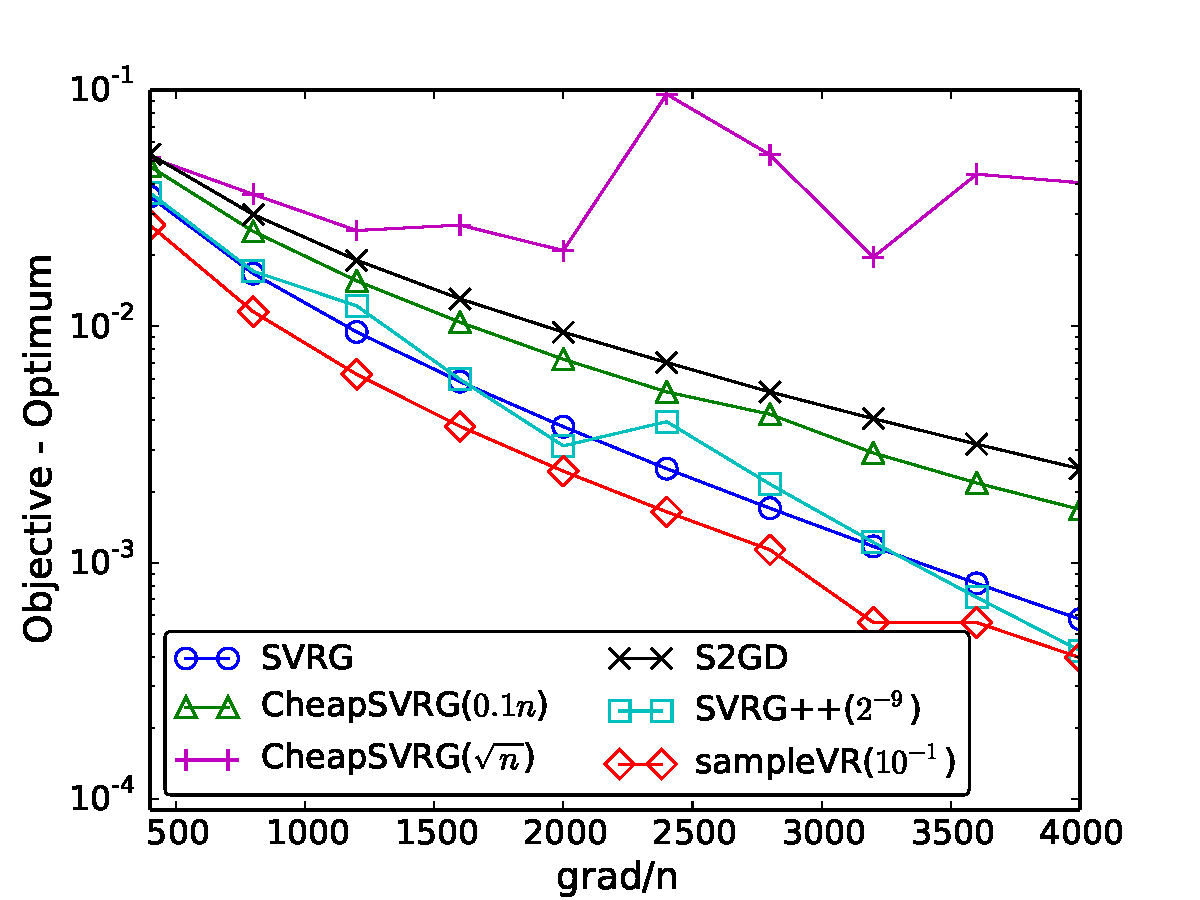
\includegraphics[width=0.5\columnwidth]{figure_ijcnn_convergence}\label{figure_ijcnn_convergence}}
\subfigure[colon-cancer]{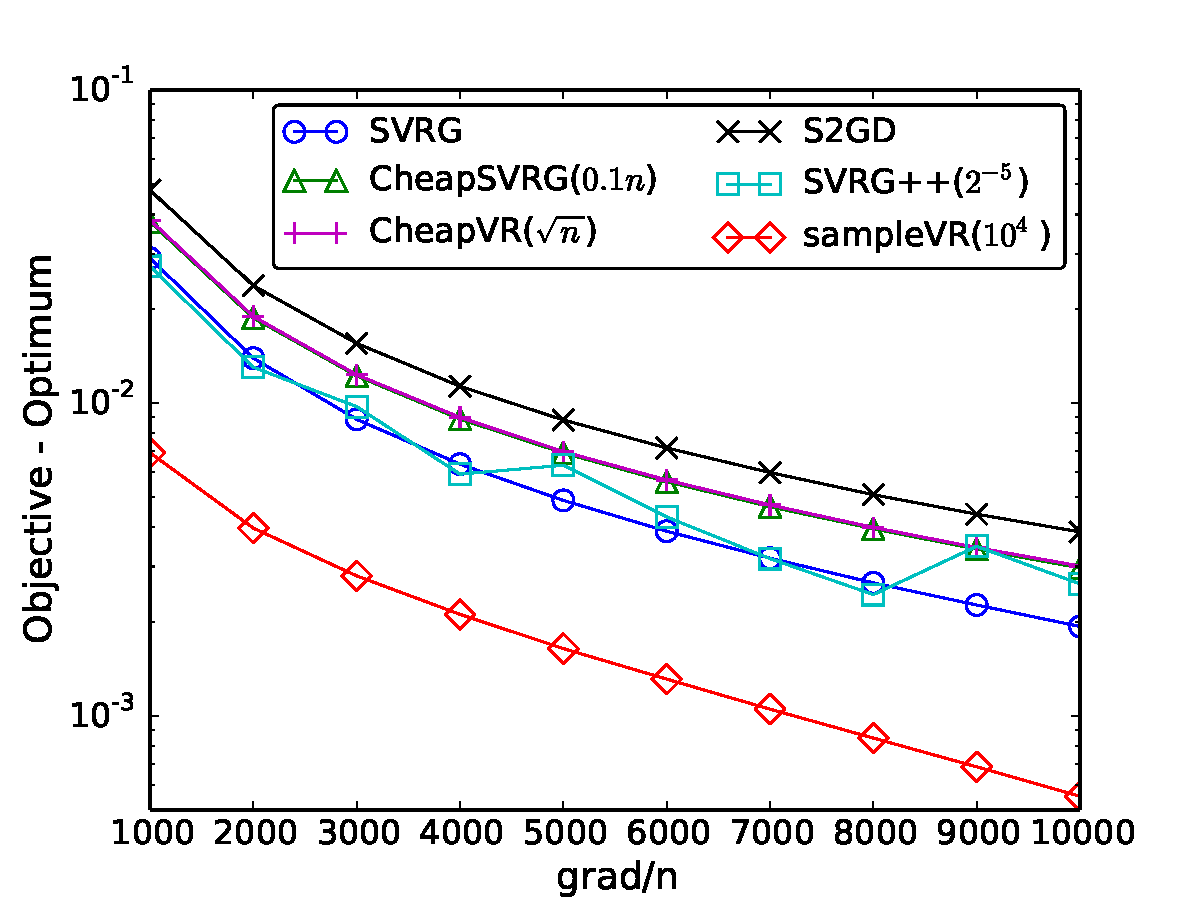
\includegraphics[width=0.5\columnwidth]{figure_colon-cancer_convergence}\label{figure_colon-cancer_convergence}}
\subfigure[duke-breast-cancer]{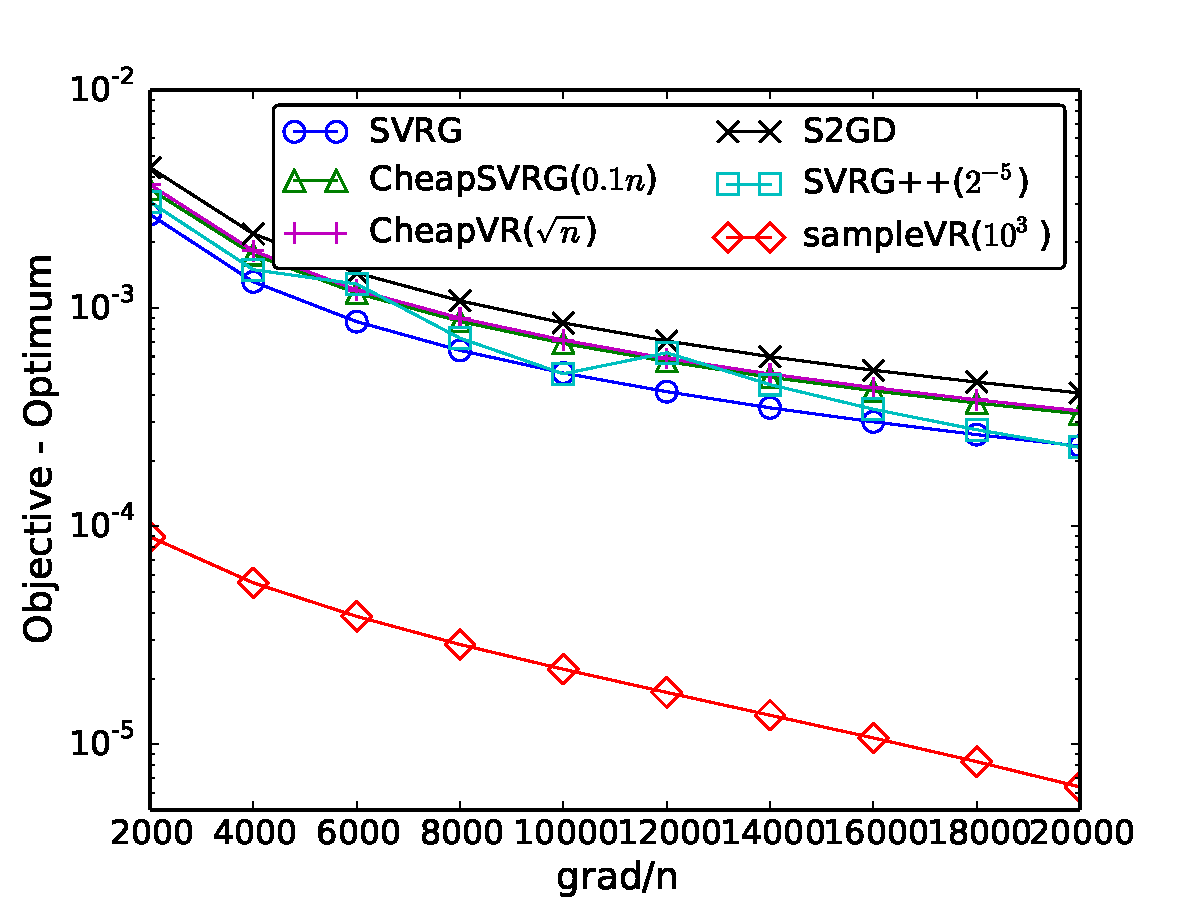
\includegraphics[width=0.5\columnwidth]{figure_duke_convergence}\label{figure_duke_convergence}}
\subfigure[a9a]{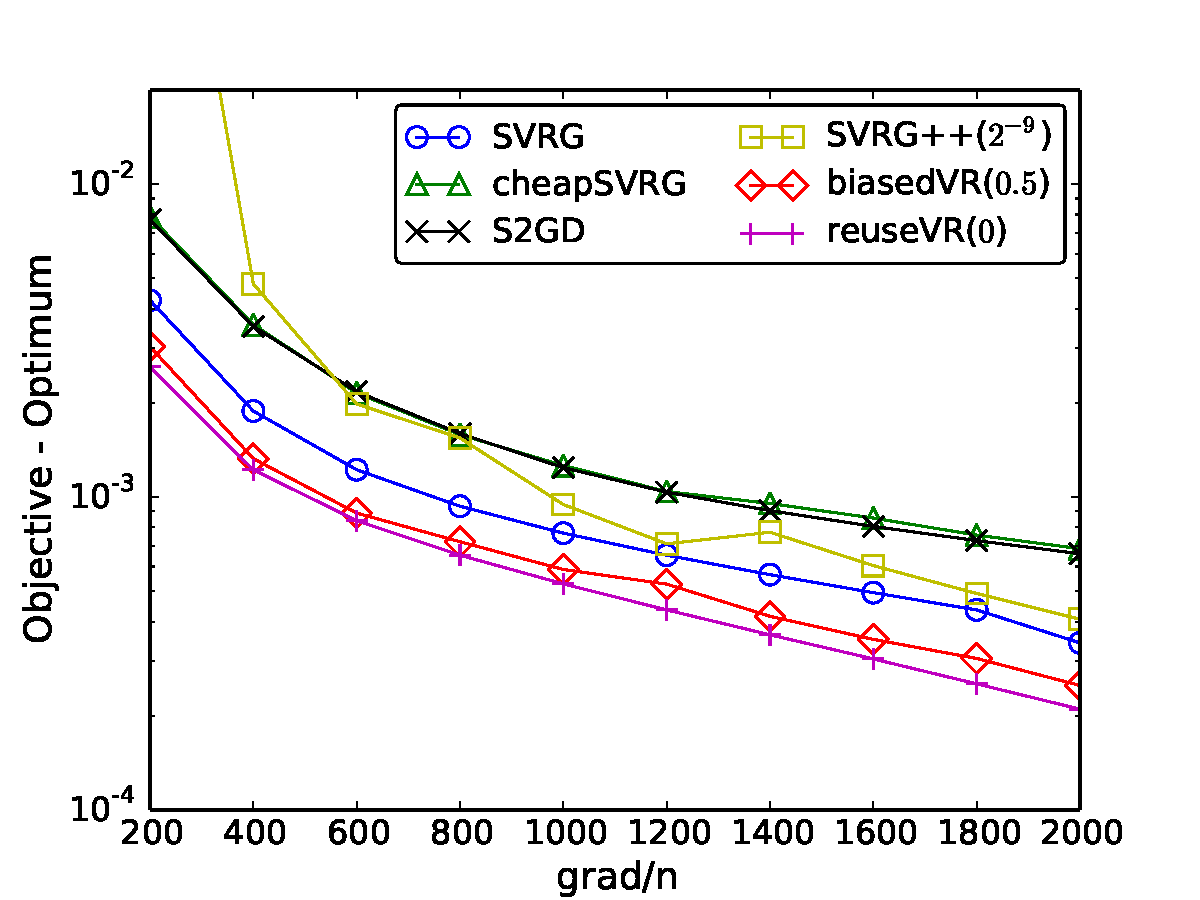
\includegraphics[width=0.5\columnwidth]{figure_a9a_convergence}\label{figure_a9a_convergence}}
\caption{\textsc{sampleVR} makes the training loss of the $l2$-regularised logistic regression tasks converge faster than the other existing algorithms.}
\label{figure_logistic_regression_convergence}
\end{figure*}

\begin{figure*}[t]
\centering
\subfigure[ijcnn1]{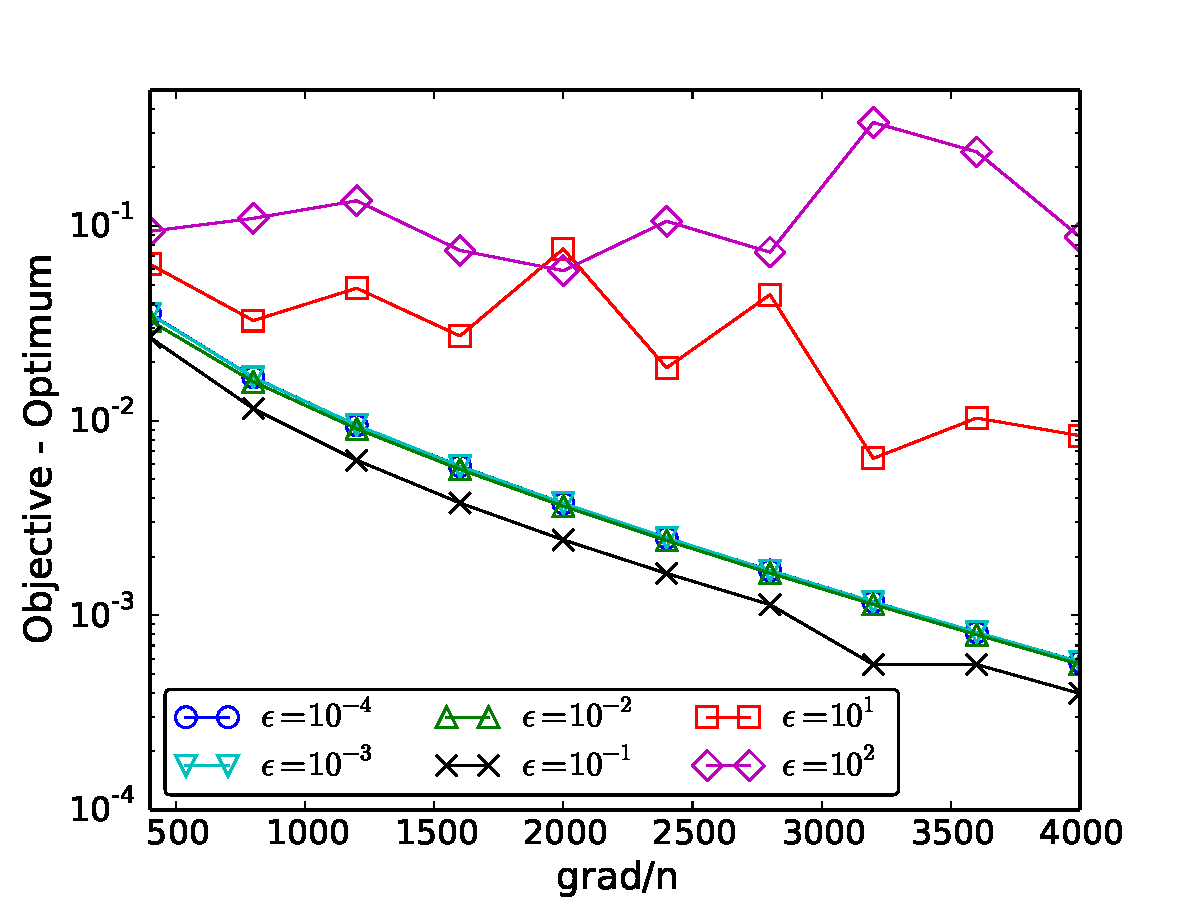
\includegraphics[width=0.5\columnwidth]{figure_ijcnn_rho}\label{figure_ijcnn_rho}}
\subfigure[colon-cancer]{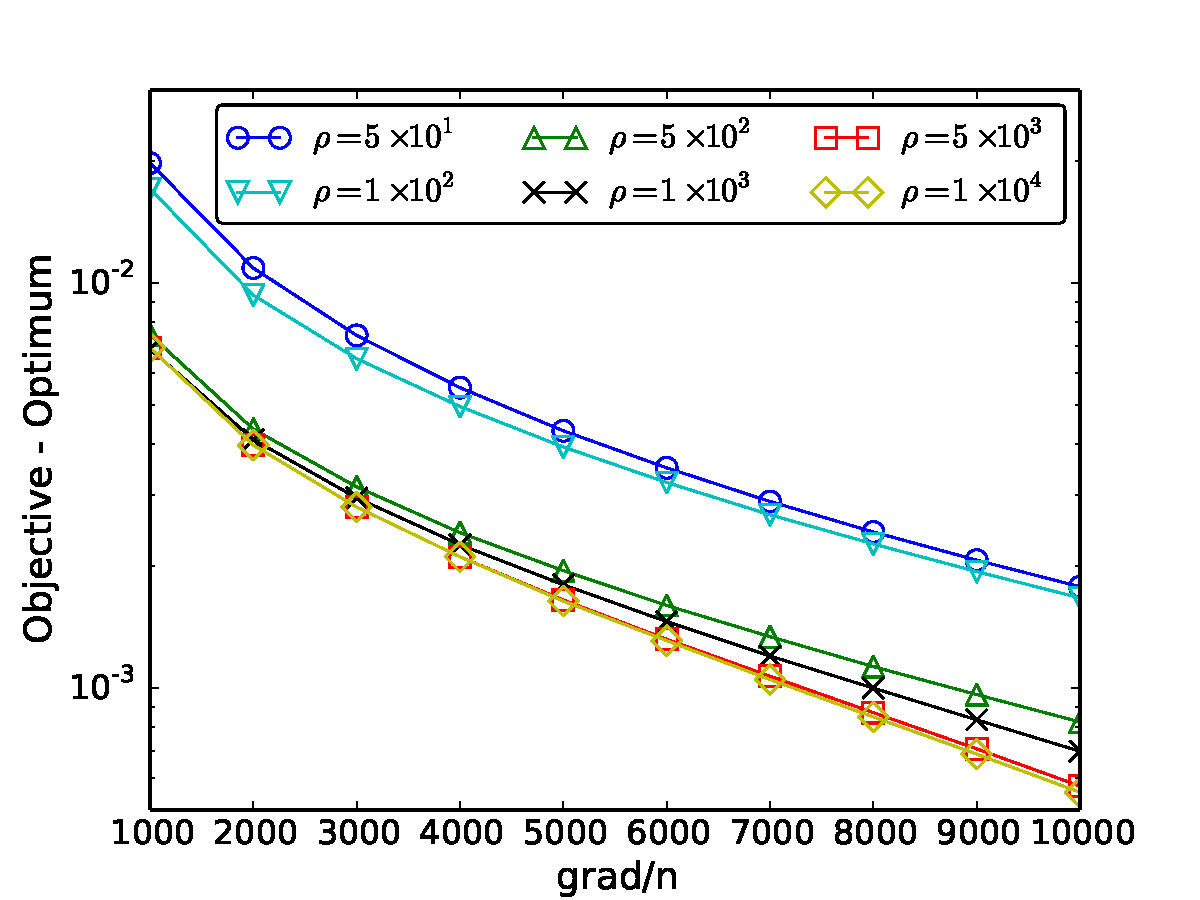
\includegraphics[width=0.5\columnwidth]{figure_colon-cancer_rho}\label{figure_colon-cancer_rho}}
\subfigure[duke-breast-cancer]{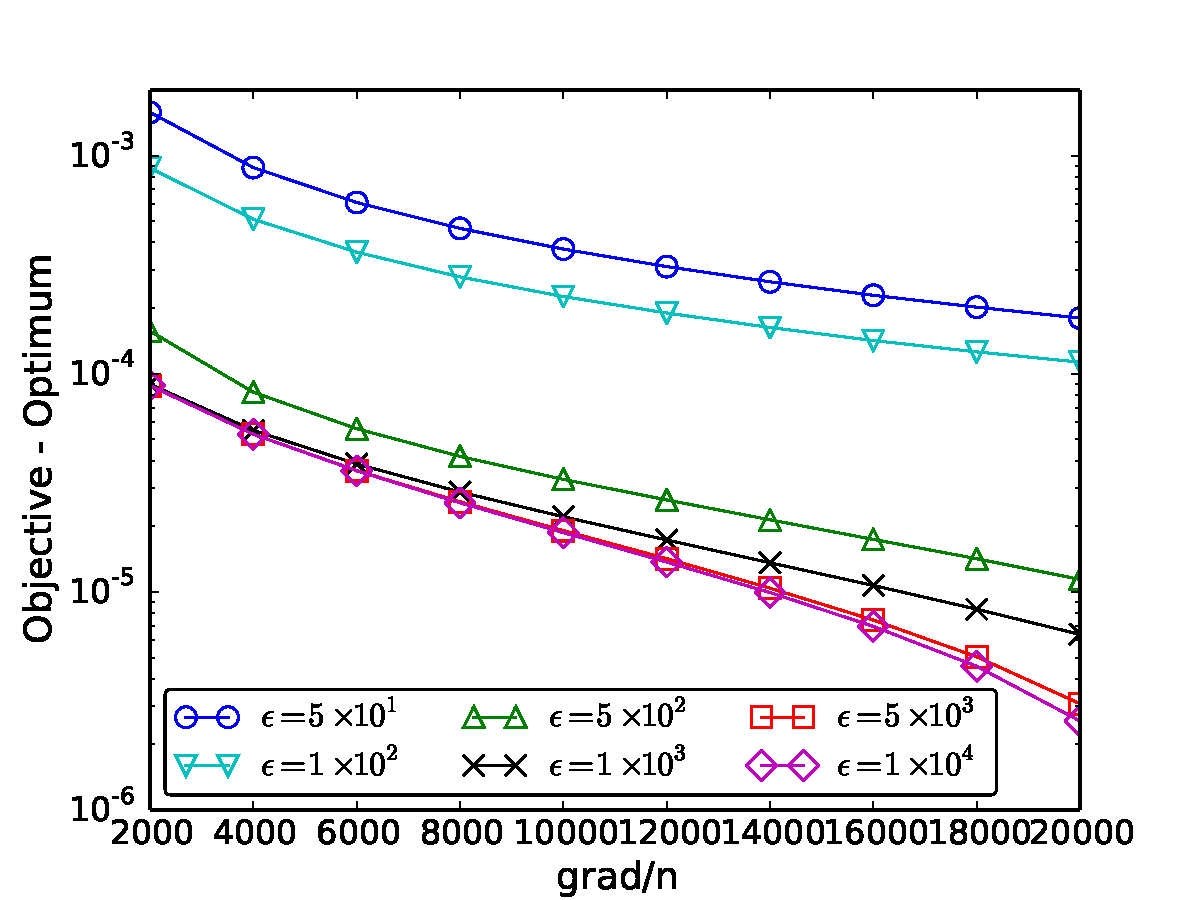
\includegraphics[width=0.5\columnwidth]{figure_duke_rho}\label{figure_duke_rho}}
\subfigure[a9a]{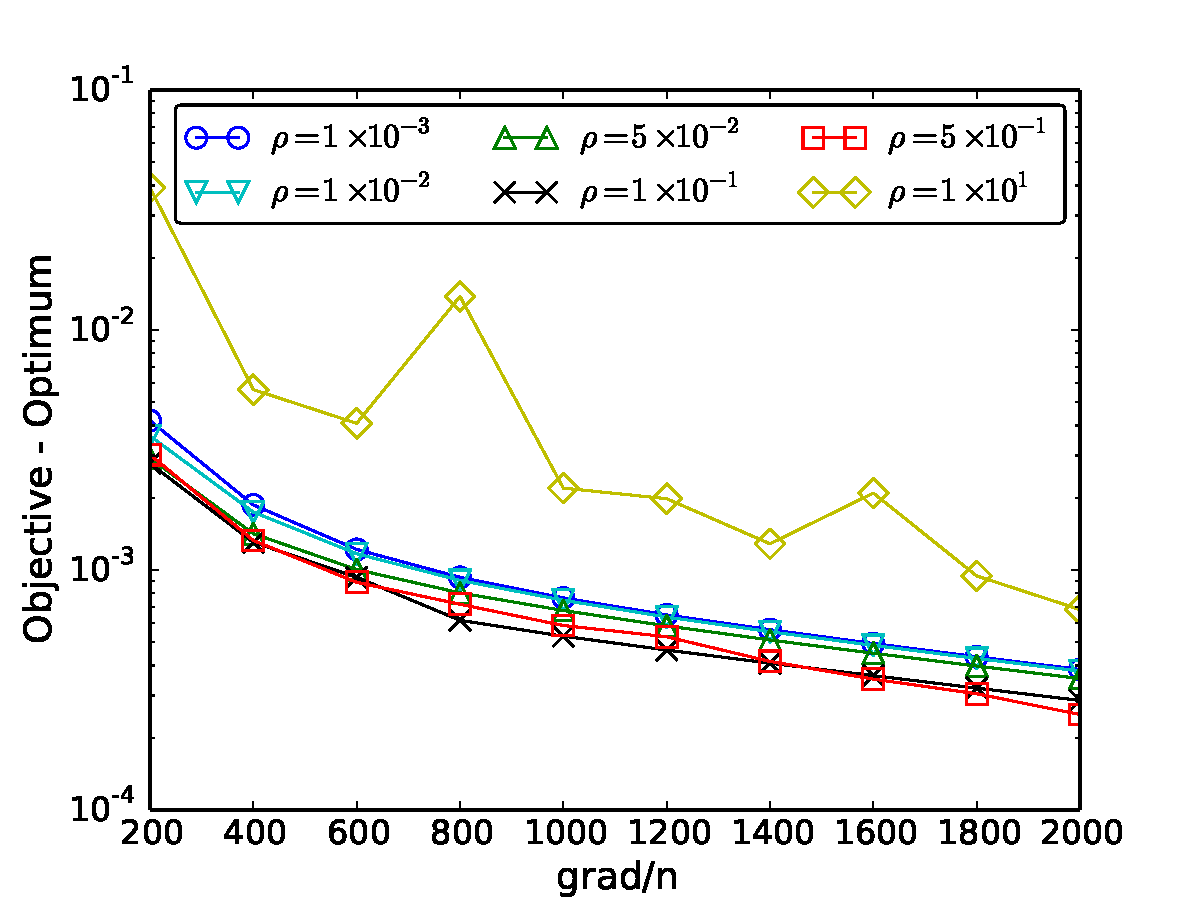
\includegraphics[width=0.5\columnwidth]{figure_a9a_rho}\label{figure_a9a_rho}}
\caption{Generally, \textsc{sampleVR} with a large $\epsilon$ has a better performance for the the $l2$-regularised logistic regression tasks. However,  the increase of the variance caused by an extremely large $\epsilon$ slows the convergence of the training loss.}
\label{figure_logistic_regression_rho}
\end{figure*}

\begin{Assumption}
Each a function $f_i$ with $i\in\{1,2, ..., n\}$ in Equ. 1 is $L$-Liptchiz continuous, that is, for any two parameters $\omega_i$ and $\omega_j$:
\label{assumption_liptchiz}
\begin{equation}
\label{equa_l_smooth} 
f_i(\omega_i)\le f_i(\omega_j)\mathrm{+}\nabla f_i(\omega_j)^\mathrm{T} (\omega_i\mathrm{-}\omega_j)\mathrm{+}\frac{L}{2}\parallel \omega_i\mathrm{-}\omega_j\parallel^2
 \end{equation}.

\end{Assumption}

\begin{Assumption}
\label{assumption_strongly_convex}
The function $F$ in Equ. 1 is $\mu$-strongly convex, that is, for any two parameters $\omega_i$ and $\omega_j$:
\begin{equation}
\label{equa_gamma_convex} 
F(\omega_i)\ge F(\omega_j)\mathrm{+}\nabla F(\omega_j)^\mathrm{T} (\omega_i\mathrm{-}\omega_j)\mathrm{+}\frac{\mu}{2}\parallel \omega_i\mathrm{-}\omega_j\parallel^2
\end{equation}.

\end{Assumption}

\begin{Theorem}
\label{theorem_converge}
$\omega_\ast$ denotes the optimum of the parameter.  $m$ can be large enough, so that $\delta = \frac{8 L \eta^2 m}{ \eta(1\mathrm{-}2\eta L) m  \mathrm{-}  \frac{1}{\mu}    }     <1$, \textsc{sampleVR} makes the optimisation objective converge linearly as:
$F(\tilde{\omega}_{s\mathrm{+}1}) \mathrm{-} F(\omega_\ast)  \le \delta [F(\tilde{\omega}_s)\mathrm{-}F(\omega_\ast)]$.
\end{Theorem}


\begin{Theorem}
\label{theorem_gradient_complexity}
\textsc{sampleVR} requires at least  $\frac{\ln \zeta}{\ln \delta}m\mathrm{+}\left( \mathrm{-} \frac{\log\frac{\alpha}{2}}{2\epsilon} (\frac{\ln \zeta}{\ln \delta}\mathrm{+}1)(\frac{\ln \zeta}{\ln \delta})\right)$ atomic gradient calculations with $\delta \mathrm{=} \frac{8 L \eta^2 m}{ \eta(1\mathrm{-}2\eta L) m  \mathrm{-}  \frac{1}{\mu}    }$ to achieve $F(\tilde{\omega}_s)\mathrm{-}F(\omega_\ast) \mathrm{\le} \zeta [F(\omega_0)\mathrm{-}F(\omega_\ast)]$.
\end{Theorem}

 As illustrated in Theorem \ref{theorem_converge} and Theorem \ref{theorem_gradient_complexity}, \textsc{sampleVR} makes the optimisation objective converge at a linear rate. To be honest,  the convergence performance is  not the best when comparing with SVRG and its variants. However, \textsc{sampleVR}
 has a significant advantage on the gradient complexity according to Theorem \ref{theorem_gradient_complexity}. For example, when the optimisation objective is strongly convex, and achieves $F(\tilde{\omega}_s)\mathrm{-}F(\omega_\ast) \le \zeta [F(\omega_0)\mathrm{-}F(\omega_\ast)]$, the gradient complexity of SVRG and its variants is $O\left(\left(n+\frac{L}{\mu}\right)\left( \frac{\ln \zeta}{\ln \delta}\right)\right)$ with $m=\frac{L}{\mu}$ \cite{Allen2015UniVR}. But, the gradient complexity of \textsc{sampleVR}  is $O\left(\left(\mathrm{-} \frac{\log\frac{\alpha}{2}}{2\epsilon} (\frac{\ln \zeta}{\ln \delta}+1)+\frac{L}{\mu} \right )\left( \frac{\ln \zeta}{\ln \delta}\right)  \right)$ with $m=\frac{L}{\mu}$. Considering $\ln n \ll n$ with $\zeta=\frac{1}{n}$, \textsc{sampleVR}  outperforms SVRG and its variants on the gradient complexity obviously.



\section{Performance evaluation}
\label{sect_performance_evaluation}

%\begin{figure*}[t]
%\centering
%\subfigure[ijcnn1]{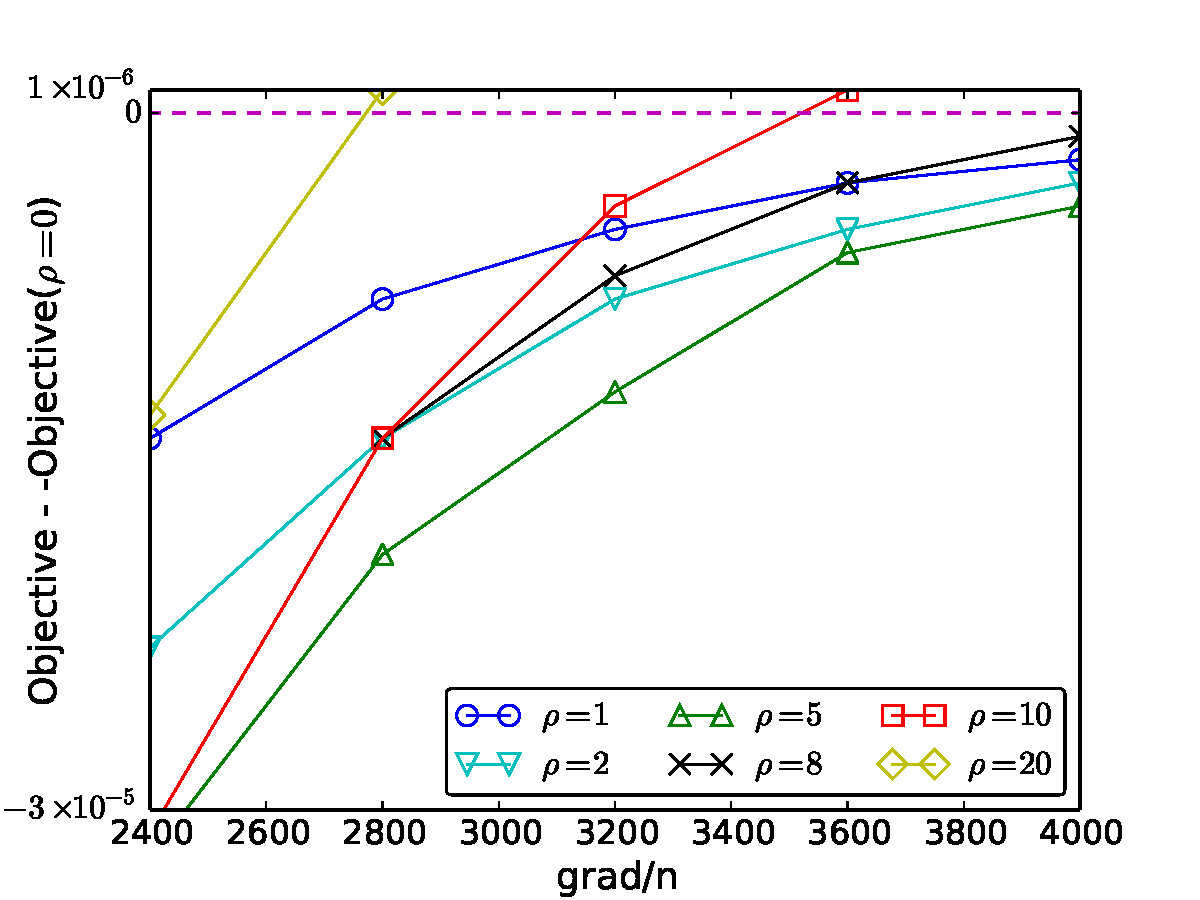
\includegraphics[width=0.5\columnwidth]{figure_ijcnn_rate}\label{figure_ijcnn_rate}}
%\subfigure[colon-cancer]{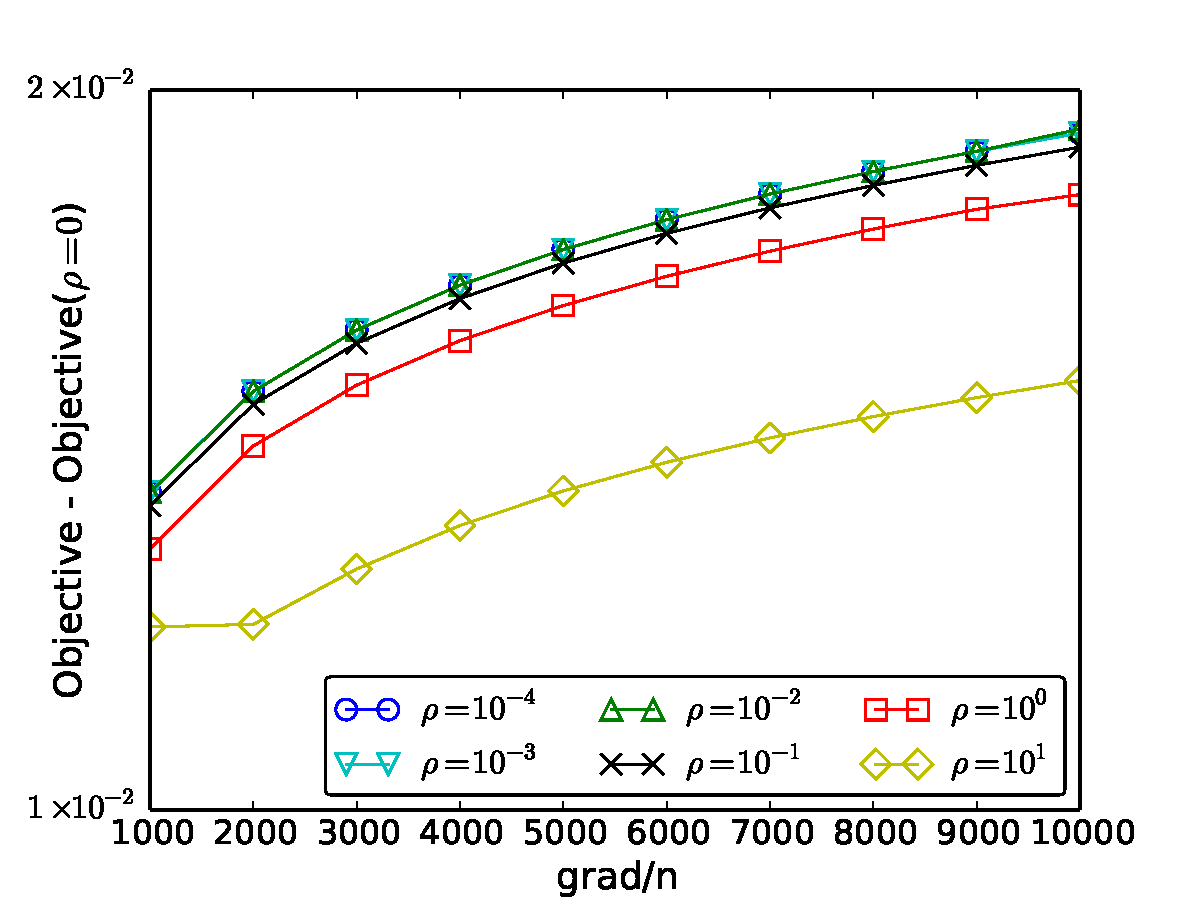
\includegraphics[width=0.5\columnwidth]{figure_colon-cancer_rate}\label{figure_colon-cancer_rate}}
%\subfigure[duke-breast-cancer]{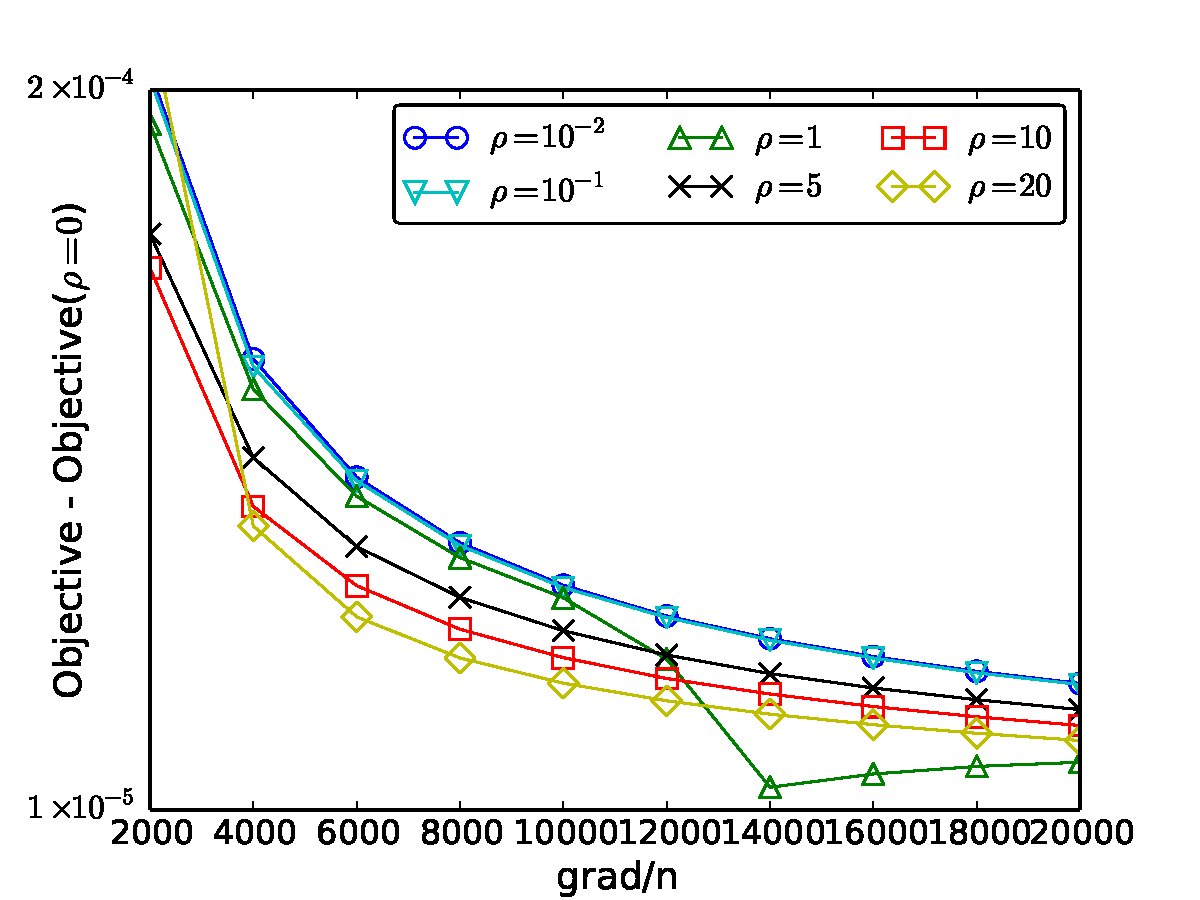
\includegraphics[width=0.5\columnwidth]{figure_duke_rate}\label{figure_duke_rate}}
%\subfigure[a9a]{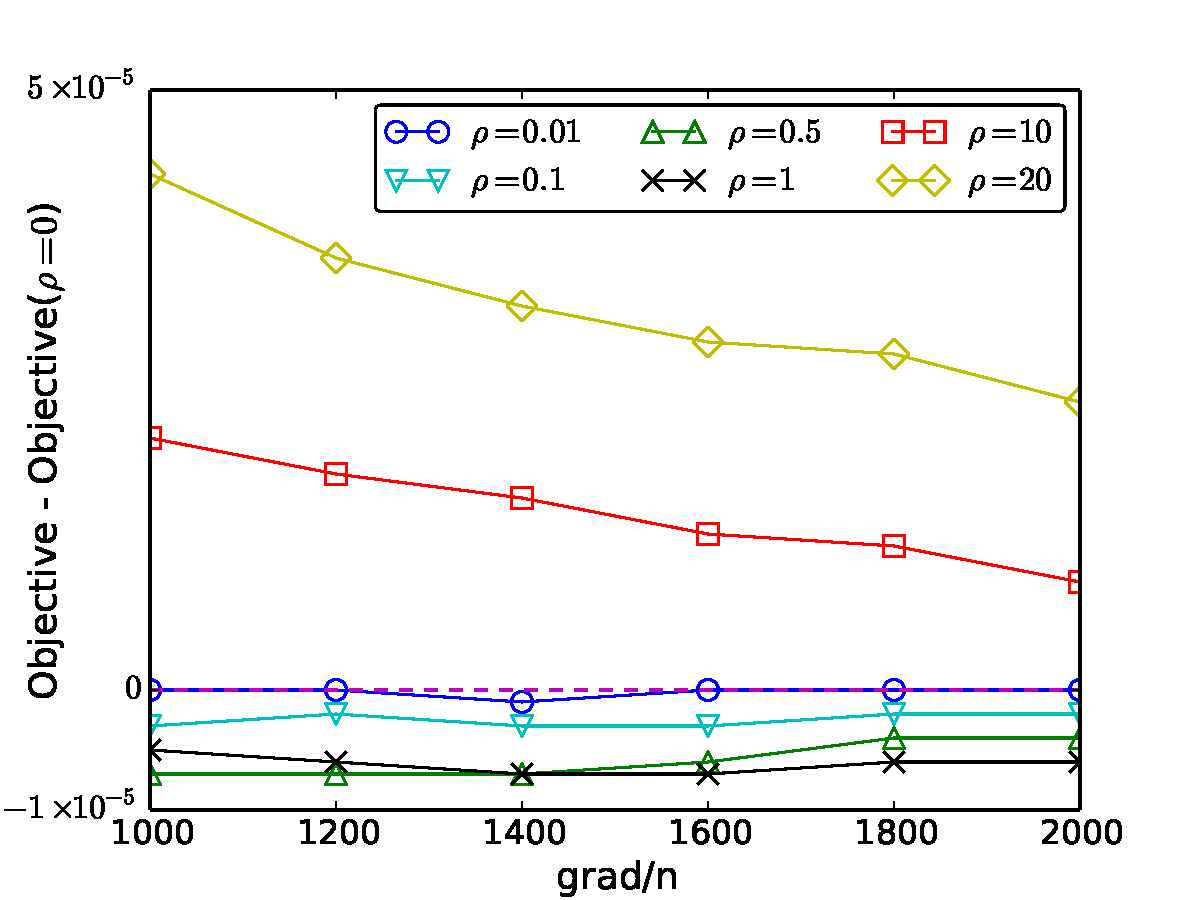
\includegraphics[width=0.5\columnwidth]{figure_a9a_rate}\label{figure_a9a_rate}}
%\caption{reuseVR}
%\label{figure_logistic_regression_rate}
%\end{figure*}



\begin{figure*}[t]
\centering
\subfigure[mg]{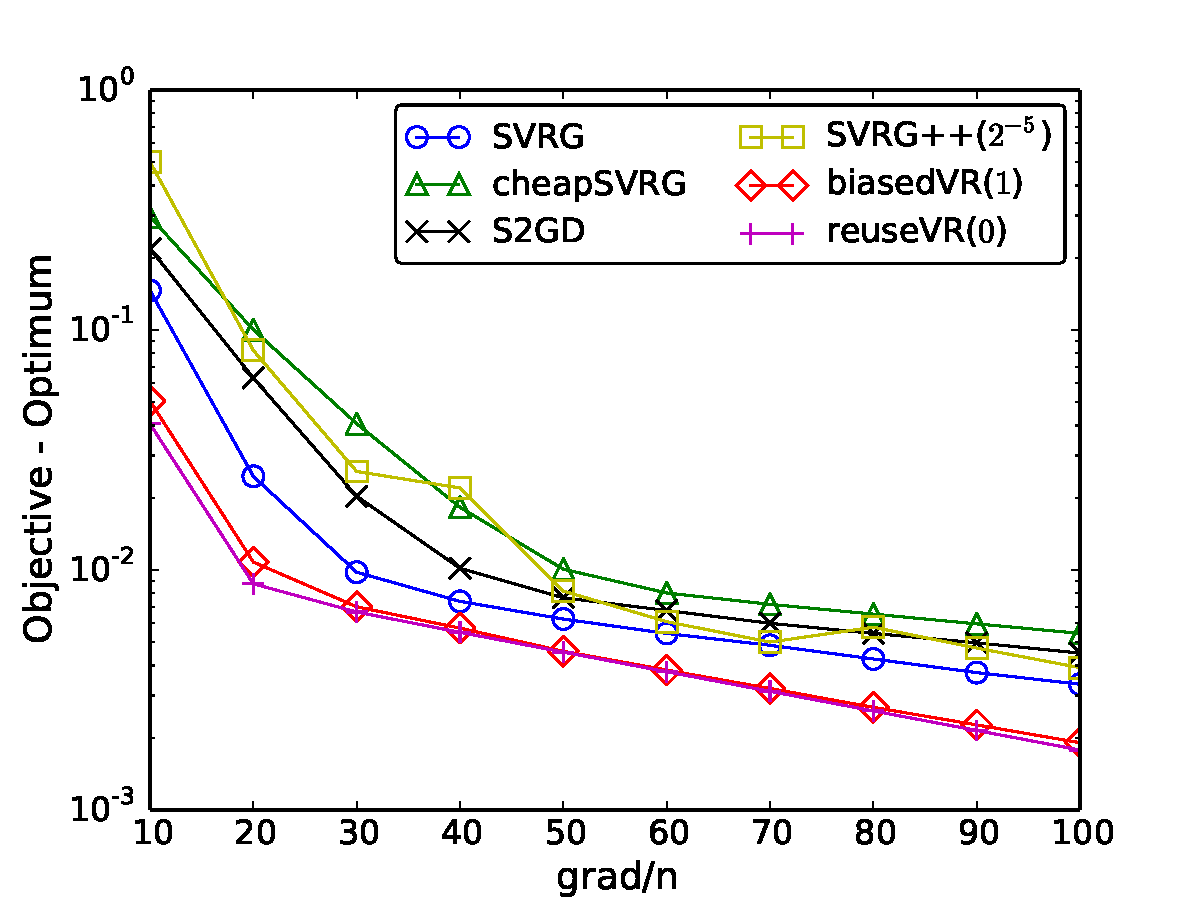
\includegraphics[width=0.5\columnwidth]{figure_mg_convergence}\label{figure_mg_convergence}}
\subfigure[cpusmall]{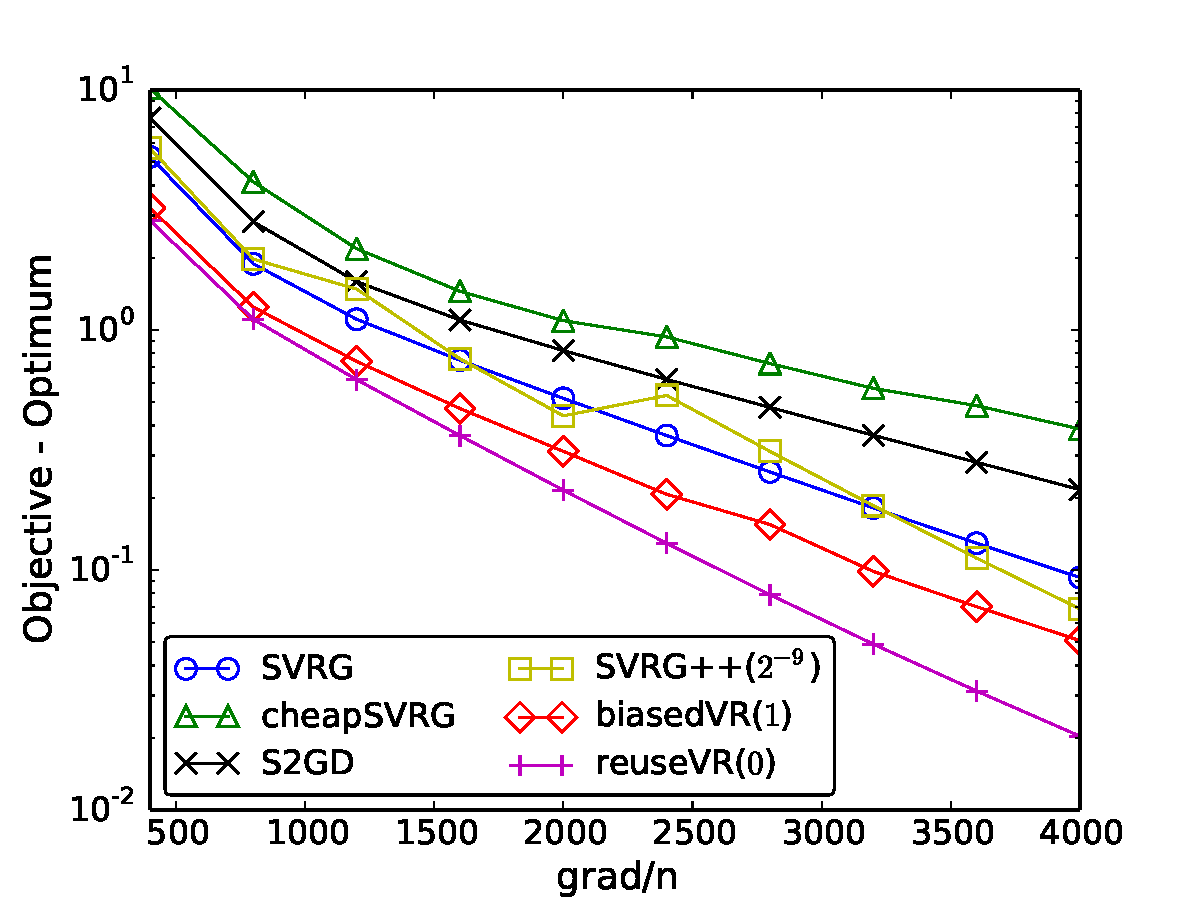
\includegraphics[width=0.5\columnwidth]{figure_cpusmall_convergence}\label{figure_cpusmall_convergence}}
\subfigure[yearPredictionMSD]{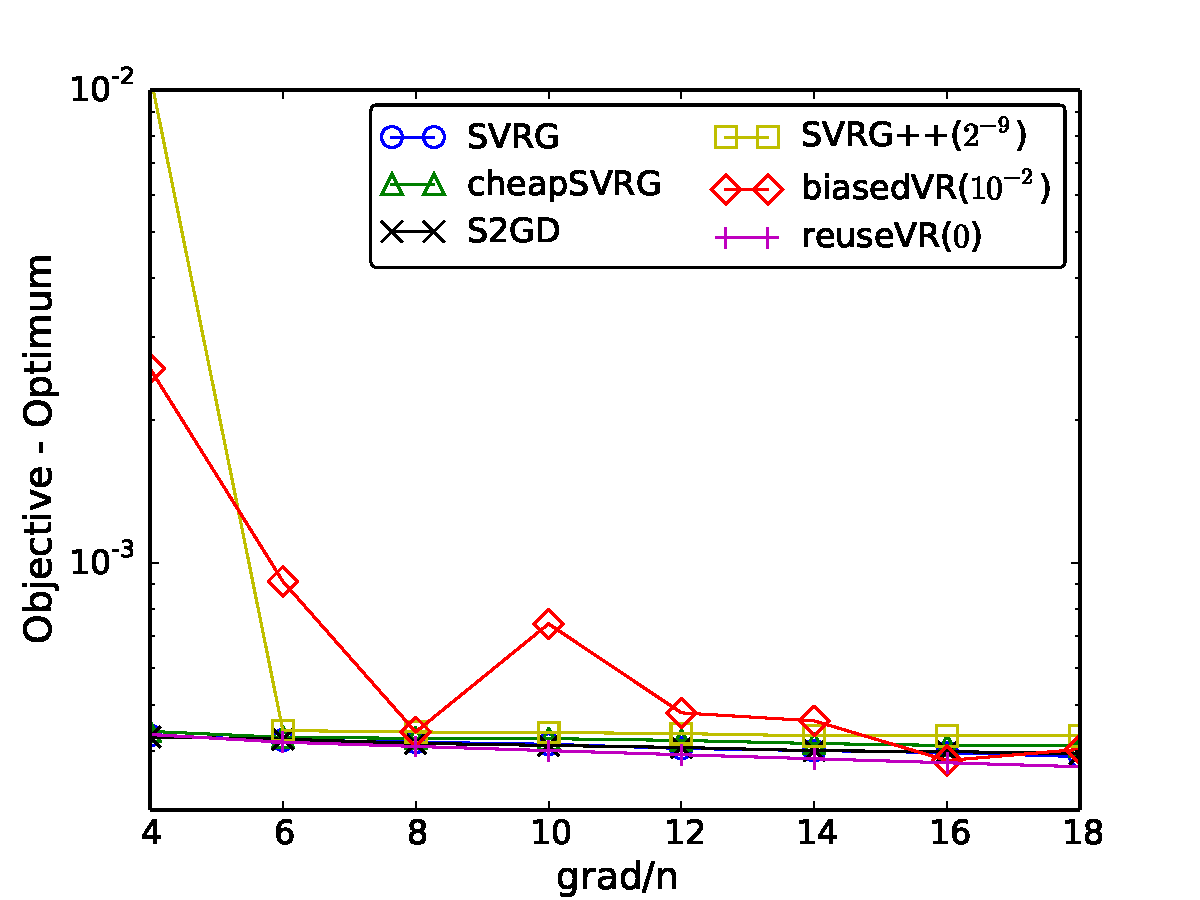
\includegraphics[width=0.5\columnwidth]{figure_year_convergence}\label{figure_year_convergence}}
\subfigure[space-ga]{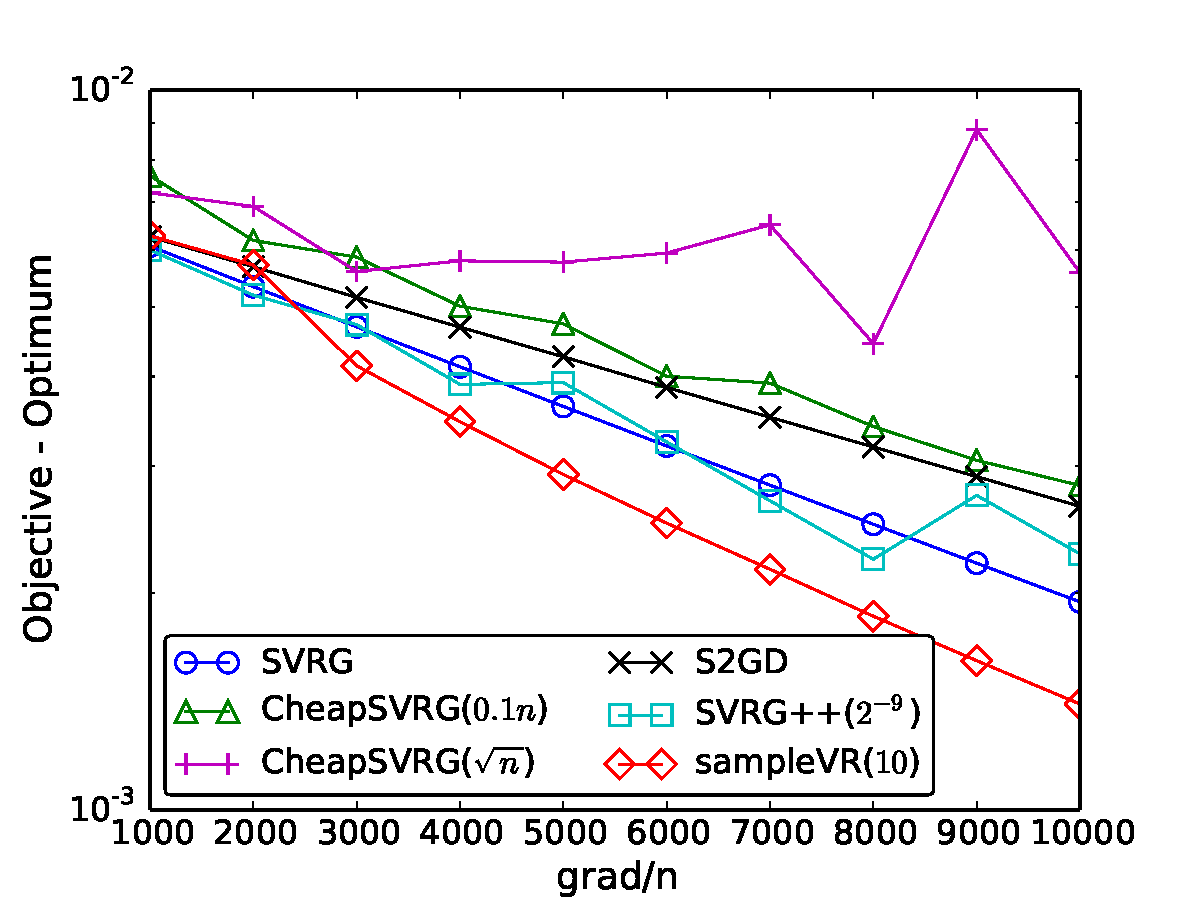
\includegraphics[width=0.5\columnwidth]{figure_space-ga_convergence}\label{figure_space-ga_convergence}}
\caption{Generally, \textsc{sampleVR}  outperforms the other existing algorithms on the convergence of the training loss when conducting the ridge regression tasks.}
\label{figure_ridge_regression_convergence}
\end{figure*}



\begin{figure*}[t]
\centering
\subfigure[mg]{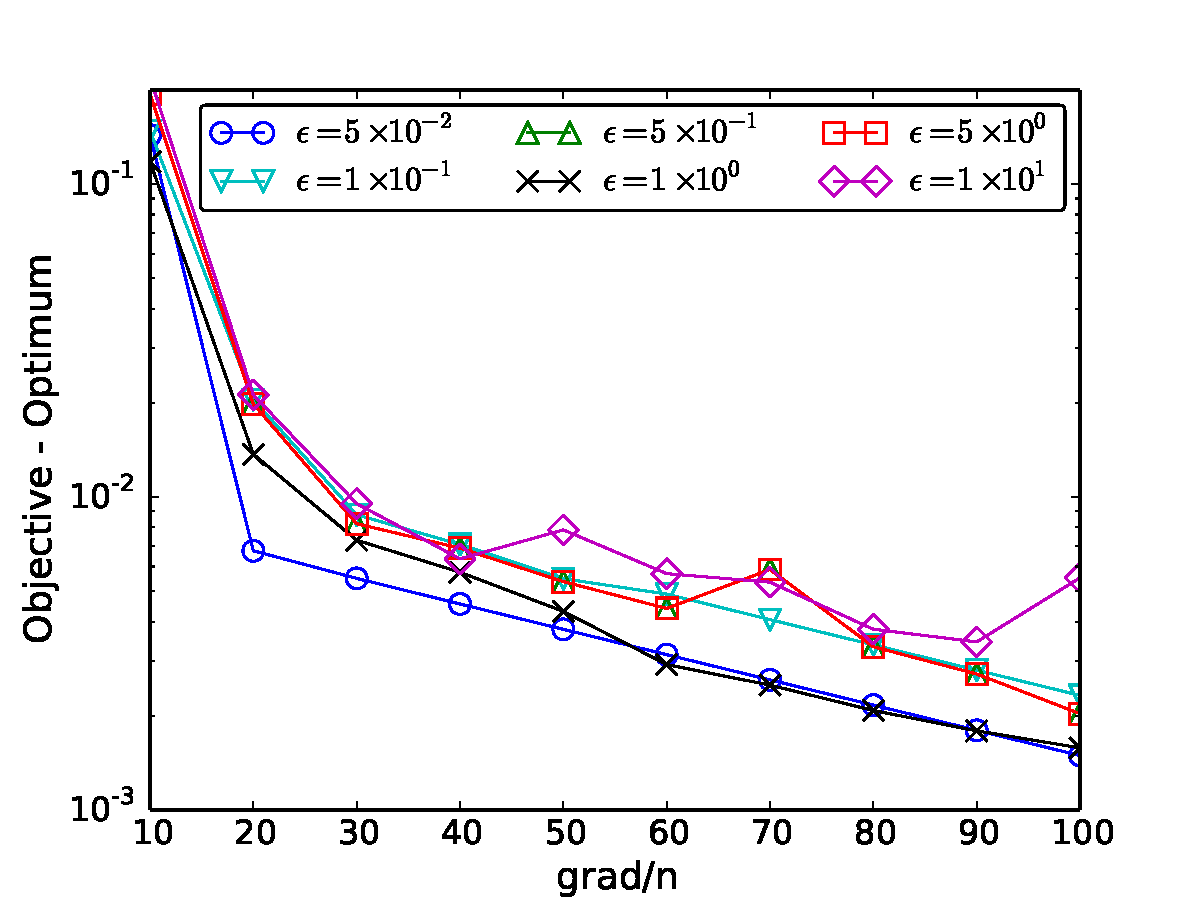
\includegraphics[width=0.5\columnwidth]{figure_mg_rho}\label{figure_mg_rho}}
\subfigure[cpusmall]{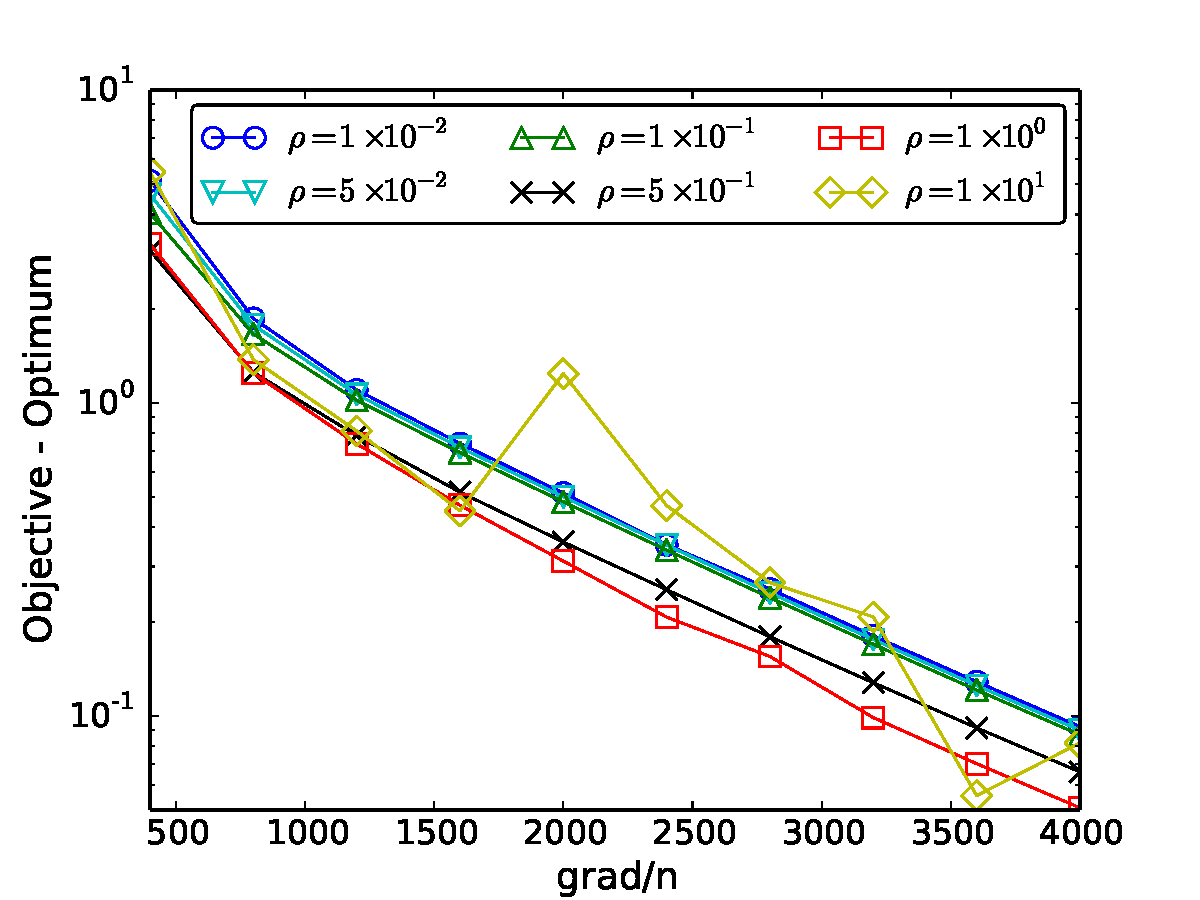
\includegraphics[width=0.5\columnwidth]{figure_cpusmall_rho}\label{figure_cpusmall_rho}}
\subfigure[yearPredictionMSD]{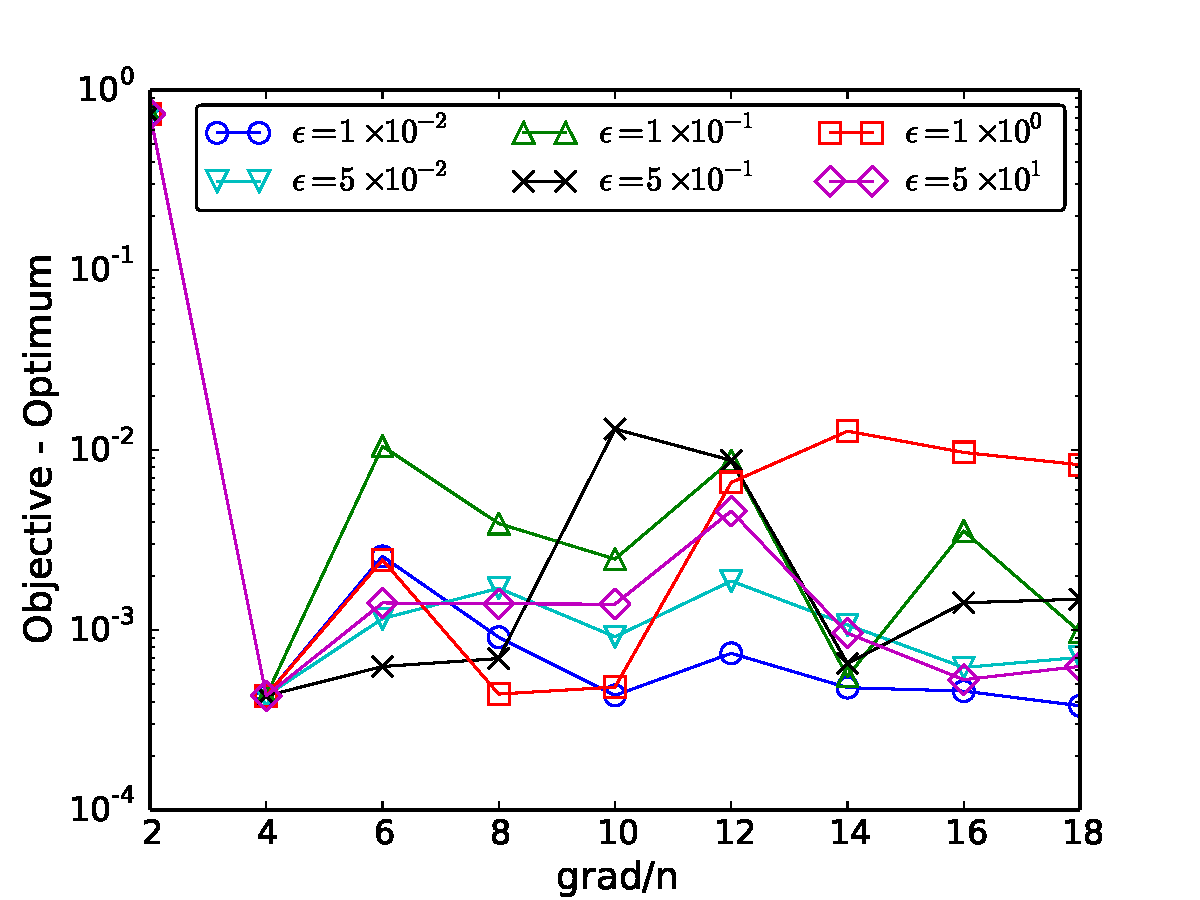
\includegraphics[width=0.5\columnwidth]{figure_year_rho}\label{figure_year_rho}}
\subfigure[space-ga]{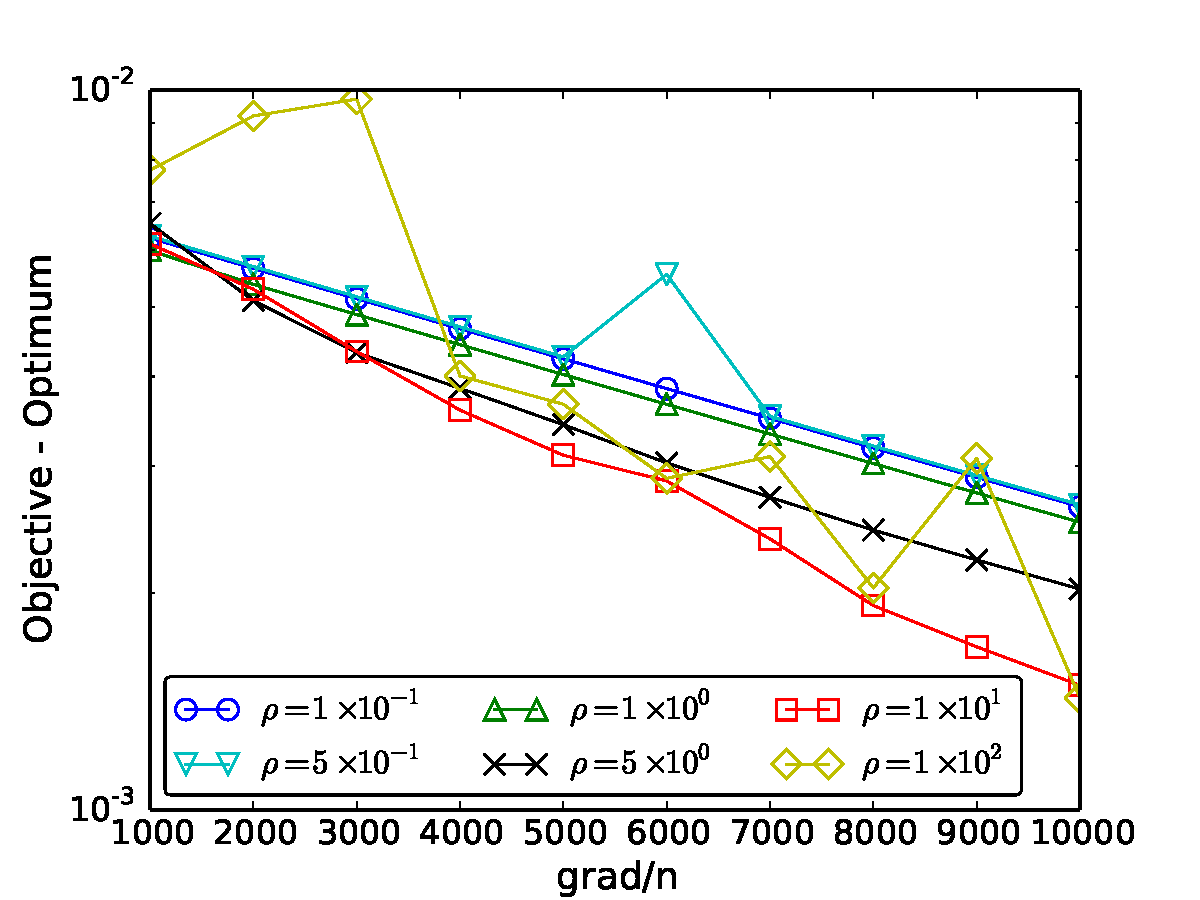
\includegraphics[width=0.5\columnwidth]{figure_space-ga_rho}\label{figure_space-ga_rho}}
\caption{A large $\epsilon$ leads to the fast convergence of the training loss for \textsc{sampleVR} when conducting the ridge regression tasks. However, the performance of  \textsc{sampleVR} is impaired  due to the increase of variance when $\epsilon$ is set to be too large.}
\label{figure_ridge_regression_rho}
\end{figure*}



\subsection{Experimental settings}
\label{sect_experimental_settings}
The existing variants of SGD with the variance reduction technique, including SVRG, S2GD, SVRG++, \textsc{CheapSVRG} have been used to conduct the performance evaluation with our proposed algorithm, i.e. \textsc{sampleVR}. The number of sampled instances in \textsc{CheapSVRG} is identified as $0.1n$ and $\sqrt{n}$ where $n$ represents the size of the training data.
Those algorithms are evaluated on eight datasets, including ijcnn1, colon-cancer, duke-brease-cancer, a9a, mg, cpusmall, yearPredictionMSD, and space-ga. All of those datasets are public on the LibSVM website \footnote{http://www.csie.ntu.edu.tw/$\sim$cjlin/libsvmtools/datasets/}. 

First, those algorithms are compared by conducting the $l2$-regularised logistic regression tasks on the datasets: ijcnn1, colon-cancer, duke-breast-cancer, and a9a. When the label of an instance is set to be $1$ or $-1$, the loss function of the $l2$-regularised logistic regression tasks is:
\begin{equation}
\label{standard_sgd}
\min\limits_\omega \frac{1}{n}\sum\limits_{i=1}^n \log(1+e^{-y_i \omega^\mathrm{T} x_i }) + \lambda \parallel \omega \parallel^2
\end{equation}. Second, we compare those algorithms by conducting ridge regression tasks on the other four datasets, i.e. mg, cpusmall, yearPredictionMSD, and space-ga. The loss function of the ridge regression tasks is:
\begin{equation}
\label{standard_sgd}
\min\limits_\omega \frac{1}{n}\sum\limits_{i=1}^n\left(\omega^{\mathrm{T}}x_i-y_i\right)^2 + \lambda \parallel \omega \parallel^2
\end{equation}. We set $\lambda$ to be $10^{-5}$, and the learning rate, i.e. $\eta$ to be $10^{-4}$ for all the evaluation tests.  The epoch size $m_s$ in SVRG and \textsc{CheapSVRG} is set to be the size of the training data, i.e. $m_s=n$. The maximal epoch size in S2GD is set to be the size of the training data, i.e. $n$.    The x-axis in all  figures of the evaluation tests represents the computational cost. The computational cost is measured by the number of gradient computations divided by  the size of the training data, i.e. $n$. The y-axis in all the figures denotes the training loss residual which is the training loss minus the optimum. Here, the optimum is estimated by running the gradient descent for a long time. The value in the bracket of the legend of SVRG++ and \textsc{sampleVR} represents the initial epoch size divided by the size of the training data, i.e. $n$ and $\epsilon$ according to Algorithm \ref{algorithm_sampleVR}, respectively.

\subsection{$l2$-regularised logistic regression}
\label{sect_performance_evaluation_convergence}
As illustrated in Figure \ref{figure_logistic_regression_convergence}, we compare the performance of all the algorithms by conducting the $l2$-regularised logistic regression tasks.  It is obvious that our proposed algorithm, i.e. \textsc{sampleVR} makes the training loss converge linearly, and outperforms other existing algorithms.   The main reason is that  \textsc{sampleVR} replaces  the computation of the full gradient with an estimation, thus getting rid of the time-consuming calculations of the gradient.  Although the estimation of the full gradient is used in  \textsc{CheapSVRG}, the number of sampled instances in \textsc{CheapSVRG} is determined as a constant such as $\sqrt{n}$, leading to much variance. Benefiting from the increase of the number of sampled instances,  \textsc{sampleVR} reduces the variance over epochs, and thus outperforms \textsc{CheapSVRG} . 
Additionally, the comparison of the  performance of \textsc{sampleVR} by varying   $\epsilon$ is shown  in Figure \ref{figure_logistic_regression_rho}. \textsc{sampleVR} generally obtains a better performance with a larger $\epsilon$. It is because that the number of the required sampled instances becomes small with a large $\epsilon$ according to Equ. \ref{equ_estimate_samples_lower_bound}, which  leads to the acceleration of \textsc{sampleVR}. However, as illustrated in Figure \ref{figure_ijcnn_rho} and \ref{figure_a9a_rho}, if $\epsilon$ is set to be too large, the performance will be impaired due to the variance between the full gradient and the estimation. In specific, a very large $\epsilon$  means that the number of the sampled instances becomes extremely small, leading to much variance between the full gradient and the estimation,  which slows the convergence of the training loss. 

\subsection{Ridge regression}
\label{sect_performance_evaluation_convergence}
As illustrated in Figure \ref{figure_ridge_regression_convergence}, we report the comparison of the performance by using all the algorithms to  conduct  ridge regression tasks. \textsc{sampleVR} has a better performance for the datasets mg, cpusmall, and space-ga than the existing algorithms significantly. The main reason is that \textsc{sampleVR} uses an unbiased estimation of the full gradient, instead of costing much time to compute it.  Although \textsc{sampleVR} does not outperform other algorithms for the dataset yearPredictionMSD at the beginning of the train process, its performance is comparable to the other algorithms, and finally shows the advantage over most of the existing algorithms. As illustrated in Figure \ref{figure_year_convergence}, the variance of the training loss by using \textsc{sampleVR} is decreased, which benefits from the increase of the sampled instances. As illustrated in Figure \ref{figure_ridge_regression_rho}, the performance of \textsc{sampleVR} has been compared by varying the value of $\epsilon$. It is significant that the variance becomes noticeable with the increase of $\epsilon$. It is because that a large $\epsilon$ leads to few sampled instances  according to Equ. \ref{equ_estimate_samples_lower_bound}, incurring much variance in the estimation of the full gradient. Moreover, as illustrated in Figure \ref{figure_mg_rho}, \ref{figure_cpusmall_rho} and \ref{figure_space-ga_rho}, an extremely small  $\epsilon$  impairs  the performance of \textsc{sampleVR}. The reason is that a small $\epsilon$ means that a large number of the instances are required to be sampled, thus incurring  much calculations of gradients. A large amount of calculations of gradients cost much time, and thus makes the convergence of the loss function slow down.  



\section{Conclusion}
\label{sect_conclusion}
This paper proposes a general framework, i.e. EUI to unify the existing variants of SVRG. After that, we explain the reason of the  variance reduction technique   from a new prospective in the framework. Additionally,  we propose a new variant of SGD with the variance reduction technique, i.e. \textsc{sampleVR} which gets rid of computing the full gradient,  thus decreasing much computational cost. The theoretical and  empirical studies show that \textsc{sampleVR} outperforms the previous work, accelerating the training loss significantly.


\bibliography{reference}
\bibliographystyle{aaai}





\end{document}
